\documentclass[10pt,conference]{IEEEtran}
\usepackage{kotex}
\usepackage{cite}
\usepackage[hidelinks]{hyperref}
\usepackage{booktabs}
\usepackage{indentfirst}
\usepackage{tcolorbox}
\usepackage{makecell}
\usepackage{graphicx}
\usepackage{pict2e}
\usepackage{picture}
\usepackage{amssymb}
\usepackage{amsmath}
\usepackage{listings}
\usepackage{caption}
\usepackage{subcaption}
\usepackage[ruled,linesnumbered]{algorithm2e}
\usepackage{multirow}
\usepackage{stfloats}
\usepackage{tabularx}
\usepackage{cuted}
\usepackage{float}
\usepackage{color}
\usepackage[flushleft]{threeparttable}
\usepackage[export]{adjustbox}
\usepackage{xcolor}
\definecolor{lightred}{rgb}{1.0, 0.7, 0.7} % 연한 빨강 (1.0 = 완전한 빨강, 0.7로 연하게 조절)
\definecolor{lightgreen}{rgb}{0.7, 1.0, 0.7} % 연한 초록 (1.0 = 완전한 초록, 0.7로 연하게 조절)

\makeatletter
\let\old@lstKV@SwitchCases\lstKV@SwitchCases
\def\lstKV@SwitchCases#1#2#3{}
\makeatother
\usepackage{lstlinebgrd}
\makeatletter
\let\lstKV@SwitchCases\old@lstKV@SwitchCases

\lst@Key{numbers}{none}{%
    \def\lst@PlaceNumber{\lst@linebgrd}%
    \lstKV@SwitchCases{#1}%
    {none:\\%
     left:\def\lst@PlaceNumber{\llap{\normalfont
                \lst@numberstyle{\thelstnumber}\kern\lst@numbersep}\lst@linebgrd}\\%
     right:\def\lst@PlaceNumber{\rlap{\normalfont
                \kern\linewidth \kern\lst@numbersep
                \lst@numberstyle{\thelstnumber}}\lst@linebgrd}%
    }{\PackageError{Listings}{Numbers #1 unknown}\@ehc}}
\makeatother

\usepackage{expl3,xparse}

\ExplSyntaxOn
\NewDocumentCommand \lstcolorlines { O{green} m }
{
 \clist_if_in:nVT { #2 } { \the\value{lstnumber} }{ \color{#1} }
}
\ExplSyntaxOff

\newcommand{\hrulealg}[0]{\vspace{1mm} \hrule \vspace{1mm}}
\newlength\mylen
\newcommand\myinput[1]{%
  \settowidth\mylen{\KwIn{}}%
  \setlength\hangindent{\mylen}%
  \hspace*{\mylen}#1\\}

\makeatletter
\DeclareRobustCommand{\Arrow}[1][]{%
\check@mathfonts
\if\relax\detokenize{#1}\relax
\settowidth{\dimen@}{$\m@th\rightarrow$}%
\else
\setlength{\dimen@}{#1}%
\fi
\sbox\z@{\usefont{U}{lasy}{m}{n}\symbol{41}}%
\begin{picture}(\dimen@,\ht\z@)
\roundcap
\put(\dimexpr\dimen@-.7\wd\z@,0){\usebox\z@}
\put(0,\fontdimen22\textfont2){\line(1,0){\dimen@}}
\end{picture}%
}
\makeatother
\newcommand{\veryshortrightarrow}{\hspace{.2mm}\scalebox{.8}{\Arrow[.1cm]}\hspace{.2mm}}

\begin{document}

\title{Automated Feedback Generation for Programming Assignments through Diversification}

\author{
    \IEEEauthorblockN{Dongwook Choi}
    \IEEEauthorblockA{
        \textit{Department of Computer Science and Engineering} \\
        \textit{Sungkyunkwan University} \\
        Suwon, Republic of Korea \\
        dwchoi95@skku.edu}

    \and

    \IEEEauthorblockN{Eunseok Lee}
    \IEEEauthorblockA{
        \textit{College of Computing and Informatics} \\
        \textit{Sungkyunkwan University} \\
        Suwon, Republic of Korea \\
        leees@skku.edu}
}

\maketitle



\begin{abstract}
    % 학생들의 프로그래밍 과제에서 즉각적이고 personalized feedback은 학생들의 프로그래밍 스킬을 향상 시키는데 매우 중요합니다. 그러나 모든 submission이 다르게 작성되기 때문에 강사가 모든 학생에게 일일이 personalized feedback을 제공하는 것은 현실적으로 어렵습니다. 이러한 문제를 해결하기 위해 Automated Feedback Generation (AFG) 기술이 제안되었습니다. AFG 기술은 wrong program의 결함을 찾고 패치를 생성하여 검증에 통과하면 피드백으로 제공합니다. 피드백을 생성하는 과정에서 AFG는 모든 테스트케이스를 통과하는 동료의 correct programs을 기반으로 wrong program의 결함과 패치를 찾습니다. 이처럼 AFG 기술은 correct programs에 의존하기 때문에 AFG의 성능을 높이기 위해서는 다양한 구조의 correct programs가 필요합니다. 그러나 소규모 프로그래밍 수업이나 online judge에 새로 업로드된 문제에서는 correct program의 다양성이 부족할 수 있습니다. In this paper, we propose \textsc{Mentored}, a new AFG for students' programming assignments through diversification. \textsc{Mentored}는 프로그램의 다양한 조합을 통해 새로운 구조의 프로그램을 만듦으로써 wrong program에 최적화된 수정을 만들면서도 correct program에 의존적인 문제를 해결합니다. 또한, 단순히 결함에 대한 수정방안 외에 wrong program이 수정되는 과정을 투명하게 피드백으로 제공합니다. 우리는 여러 최첨단 AFG approaches와 비교하여 실제 학생들의 프로그래밍 과제에 대한 평가를 수행합니다. 우리의 데이터세트는 실제 대학의 입문 programming assignments와 online judge의 programming problems의 프로그램으로 구성됩니다. 실험 결과, \textsc{Mentored}는 최첨단 AFG approaches 보다 더 높은 수정률과 더 다양한 구조의 프로그램을 생성했습니다. 또한, 우리의 방법은 일련의 수정 과정을 투명하게 제공함으로써 학생들의 프로그래밍 스킬을 향상시키고 강사들의 피드백 생성에 대한 manual effort를 줄일 수 있을 것으로 기대됩니다. 이러한 결과는 \textsc{Mentored}가 프로그래밍 교육에서 유용한 도구가 될 수 있음을 시사합니다.
    Immediate and personalized feedback on students' programming assignments is important for improving their programming skills. However, it is challenging for instructors to give personalized feedback to every student since each program is written differently. To address this problem, the Automated Feedback Generation (AFG) technique has been proposed, which identifies faults from wrong program, generates patches, and provides feedback if pass validation. AFG relies on correct programs from students to find faults and generate patches. Therefore, having diverse correct programs is important for the performance of AFG. However, in small-scale programming courses or new online judge problems, might be a lack of diversity in correct programs. In this paper, we propose \textsc{Mentored}, a new AFG for students' programming assignments through diversification. \textsc{Mentored} generates new structures of programs through various combinations of programs to generate modifications optimized for wrong programs while solving the problem of dependency on correct programs. Additionally, \textsc{Mentored} provides transparent feedback on the process of repairing wrong programs. We evaluate \textsc{Mentored} on real student programming assignments and compare it with state-of-the-art AFG approaches. Our dataset includes real university introductory programming assignments and online judge problems. Experimental results show that \textsc{Mentored} generates higher repair rates and more diverse program structures than other AFG approaches. Moreover, by providing a transparent sequence of repair processes, \textsc{Mentored} is expected to improve students' programming skills and reduce instructors' manual effort in feedback generation. These results indicate that \textsc{Mentored} can be a useful tool in programming education.
\end{abstract}



\begin{IEEEkeywords}
    Automated Program Repair, Automated Feedback Generation, Programming Assignments
\end{IEEEkeywords}



\section{Introduction}
    % 배경
    % 프로그래밍은 소프트웨어 개발의 핵심 도구일 뿐만 아니라, 학생들이 이론적 지식을 실제 문제 해결에 적용할 수 있도록 돕고, 논리적 사고와 문제 해결 능력을 함양하는 중요한 학습 도구입니다. 최근 몇 년 동안 다양한 산업 분야에서 코딩 능력에 대한 수요가 급증하면서 프로그래밍 교육의 중요성도 크게 부각되었습니다. 이에 따라 전 세계 교육 기관들은 프로그래밍 교육을 강화하고 있으며, 프로그래밍 능력은 단순한 기술을 넘어 다양한 분야에서 필수적인 역량으로 자리 잡고 있습니다. 특히, 코딩 과제는 이러한 교육 과정에서 프로그래밍 능력을 향상시키기 위한 핵심적인 역할을 담당하고 있습니다. 코딩 과제를 통해 학생들은 배운 지식을 실제로 적용해보고, 오류를 수정하며, 문제를 해결하는 과정을 경험하게 됩니다. 그러나 이러한 교육적 효과를 극대화하기 위해서는 학생들이 코딩 과제를 수행하는 과정에서 personalized feedback을 real-time으로 받는 것이 필수적입니다. 그러나 학생들의 프로그래밍 과제는 각기 다른 변수명과 알고리즘으로 구현되어, personalized feedback을 제공하는 데 많은 시간과 노력이 필요하여 강사가 학생마다 제공하기 어렵습니다. 특히, 수백 명의 학생이 동시에 수강하는 Massive Open Online Course (MOOC)와 같은 환경에서는 강사진이 모든 학생에게 personalized feedback을 제공하는 것이 현실적으로 불가능합니다. 이로 인해 많은 학생들이 자신의 코드에서 발생한 오류를 제대로 이해하지 못하고, 어떻게 수정해야 하는지 모른 채 반복적으로 같은 실수를 저지르게 됩니다. 이러한 상황은 학생들의 학습 동기와 성취감을 저하시킬 수 있으며, 궁극적으로는 프로그래밍 학습에 대한 흥미를 잃게 만들 수 있습니다.
    Programming is not only a core tool for software development but also an essential learning tool that helps students apply theoretical knowledge to real-world problem-solving, fostering logical thinking and problem-solving skills. In recent years, the demand for coding skills has surged across various industries, highlighting the importance of programming education. As a result, educational institutions worldwide are strengthening programming education, with programming skills becoming a critical competency in diverse fields beyond just technical expertise. Programming assignments play a key role in this educational process, enabling students to apply their knowledge, debug errors, and solve problems. To maximize the educational impact, students need to receive personalized feedback in real-time while working on their programming assignments. However, since each student implements their programming assignments with different variable names and algorithms, providing personalized feedback requires significant time and effort, making it challenging for instructors to provide such feedback to every student. This issue is especially pronounced in environments like Massive Open Online Courses (MOOC), where hundreds of students participate simultaneously, making it practically impossible for instructors to provide personalized feedback to everyone. As a result, many students repeatedly make the same mistakes without understanding the faults in their code or knowing how to repair them. This situation can reduce students' motivation and sense of accomplishment, ultimately leading to a loss of interest in learning programming.

    % APR
    % Automated Program Repair (APR) 기술은 프로그램 코드에서 결함을 자동으로 식별하고, 이를 수정하는 패치를 생성하며, 수정된 코드의 정확성을 검증하는 다양한 기술을 통합한 시스템입니다. APR은 주로 Open Source Software (OSS)의 결함을 자동으로 수정하기 위해 제안되었습니다. OSS의 경우, 일반적으로 전문가들이 작성한 코드로 구성되어 있으며, 코드 구조가 잘 잡혀 있고 대부분의 테스트 케이스를 통과하는 특징이 있습니다. 따라서 APR 시스템은 이러한 전문가 수준의 코드를 대상으로 효과적인 결함 수정 기능을 발휘할 수 있습니다. 그러나 APR 기술은 프로그래밍 교육에서도 큰 잠재력을 가지고 있습니다. 학생들이 작성한 프로그래밍 과제에 APR을 적용하면, 학생들의 wrong program에 대해 자동으로 수정 방안을 제시하고, 이를 통해 학생들에게 personalized feedback을 제공할 수 있습니다. 실제로 Yi 등(2017) \cite{yi2017feasibility}의 연구에서는 입문 프로그래밍 과정을 수강하는 학생들이 작성한 프로그래밍 과제를 대상으로 APR 도구들 \cite{le2011genprog, weimer2013leveraging, mechtaev2016angelix, long2016automatic}을 적용한 실험을 진행하였습니다. 그 결과, 학생들의 프로그래밍 과제는 OSS에 비해 비교적 쉬운 수준의 코드임에도 불구하고 APR 도구의 수정률이 매우 낮았습니다. 이는 APR의 데이터셋이 주로 전문가가 작성한 코드로 구성되어 있고, single location fault을 수정하는 데 초점이 맞춰져 있기 때문입니다. 반면, 학생들이 작성한 프로그램은 초보자의 프로그램이기 때문에 구조가 잘 잡혀 있지 않고, multiple location fault이 많으며, 절반 이상의 테스트 케이스를 통과하지 못합니다 \cite{yi2017feasibility}. 이러한 특성 때문에 학생들의 프로그래밍 과제에 대해서 APR 기술을 그대로 사용하는 것에는 한계가 있습니다.
    Automated Program Repair (APR) technique is a system that integrates various techniques to automatically identify faults in program, generate patches to repair them, and validate the correctness of the repaired program. APR was primarily proposed for automatically repairing faults in Open Source Software (OSS), which is typically well-structured and written by experts, passing most test cases. Therefore, APR systems are highly effective when targeting such expert-level program. However, APR also holds great potential in programming education. When applied to student programming assignments, APR can automatically suggest modifications for wrong programs, providing personalized feedback. In a study by Yi et al. (2017) \cite{yi2017feasibility}, APR tools \cite{le2011genprog, weimer2013leveraging, mechtaev2016angelix, long2016automatic} were applied to programming assignments written by students in an introductory programming course. Despite the relative simplicity of student program compared to OSS, the repair rate of the APR tool was low. This is because APR datasets primarily consist of expert-written program, focusing on single-location faults. In contrast, student programs are often poorly structured, contain multiple-location faults, and fail more than half of the test cases \cite{yi2017feasibility}. These characteristics limit the direct application of APR to programming assignments.

    % AFG
    % 이러한 한계를 극복하기 위해, APR 기술을 기반으로 한 Automated Feedback Generation (AFG) 기술이 제안되었습니다. AFG 기술은 APR 기술의 단점인 multi location fault 문제를 보완하고, 교육 환경에 적합하게 personalized feedback을 제공하기 위해 개발되었습니다. 대부분의 AFG 기술들 \cite{hu2019re, wang2018search, gulwani2018automated, li2022generating, pu2016sk_p, heo2023referent,singh2013automated,mechtaev2018semantic,ahmed2022verifix,d2016qlose,choi2021automated,song2021context,rolim2017learning,kaleeswaran2016semi}은 APR 기술과 달리 사전 정의된 템플릿 \cite{liu2019tbar}이나 결함, 패치, context 정보등을 학습한 repair 모델 \cite{li2022transrepair}을 사용하지 않습니다. 대신, AFG는 학생들이 자주 범하는 오류를 학습한 오류 모델 \cite{singh2013automated}이나, 모든 테스트 케이스를 통과한 동료의 correct program을 활용하여 wrong program을 수정합니다. AFG가 APR에 비해 높은 수정률을 가질 수 있는 이유는 correct program를 기반으로 한다는 점입니다. 학생들의 wrong program은 일반적으로 많은 결함을 포함하고 있어 testcases의 절반 이상을 통과하지 못합니다 \cite{yi2017feasibility}. 그래서 테스트케이스를 기반으로 한 fault localzation으로 결함을 식별하기 어렵습니다. 반면 correct program을 이용하여 학생들이 제출한 wrong program와 가장 유사한 구조의 correct program를 비교하면, 테스트케이스를 사용하지 않고도 결함을 식별할 수 있습니다. 이는 correct program이 존재하는 프로그래밍 과제 도메인에서만 가능한 방법으로 APR과의 차별점을 보여줍니다. AFG의 이러한 차별점으로 인해 프로그램 수정 성능이 APR에 비해 월등히 뛰어나며, 특히 학생 코드와 같이 구조가 잡혀 있지 않고 결함이 많은 코드에서도 높은 성능을 보여줍니다. 즉, correct program은 AFG의 성능에 있어 중대한 역할을 합니다.
    To overcome these limitations, Automated Feedback Generation (AFG) technique based on APR was proposed. AFG was developed to address APR's shortcomings, such as the multi-location fault issue, and to provide personalized feedback suitable for educational environments. Unlike APR, most AFG techniques \cite{hu2019re, wang2018search, gulwani2018automated, li2022generating, pu2016sk_p, heo2023referent,singh2013automated,mechtaev2018semantic,ahmed2022verifix,d2016qlose,choi2021automated,song2021context,rolim2017learning,kaleeswaran2016semi} do not use predefined templates \cite{liu2019tbar} or repair models \cite{li2022transrepair} that learn from fault, patch, and context information. Instead, AFG utilizes error models \cite{singh2013automated} that learn common mistakes made by students or compares the wrong program to peers' correct programs that have passed all test cases. The reason AFG tends to have a higher repair rate than APR is its reliance on correct programs. Since student submissions often contain many faults and fail more than half of the test cases, it is difficult to identify faults through test case-based fault localization \cite{yi2017feasibility}. However, by comparing the wrong program with the most structurally similar correct program, AFG can identify faults without relying on test cases. This method is unique to programming assignments where correct programs exist, highlighting a key distinction from APR. As a result, AFG outperforms APR, especially in handling student program of poorly structured and many faults. In essence, correct programs play a critical role in the effectiveness of AFG.

    % 문제
    % MOOC와 같이 학생 수가 많은 경우 correct program의 다양성이 보장될 수 있지만, 소규모 프로그래밍 수업이나 새로운 Online Judge 문제의 경우 correct program이 부족할 수 있습니다. \textsc{Refactory} \cite{hu2019re}는 correct program을 refactoring하여 다양한 구조의 correct program을 추가로 생성하기 때문에 다양한 correct program을 만들 수 있습니다. 그러나 \textsc{Refactory}는 최소한 1개의 correct program을 필요로 하며 refactoring이 코드의 구조나 스타일을 개선해줄 수는 있지만 새로운 알고리즘이나 접근 방법을 만들지는 않습니다. \textsc{AssignmentMender} \cite{li2022generating}는 mutation을 이용한 방법으로 correct program이 없을 때도 새로운 알고리즘의 correct program을 생성할 수 있습니다. 하지만 무작위성 수정으로 인해 의미 없는 수정을 하거나 새로운 버그를 도입할 수 있습니다. \textsc{Referent} \cite{heo2023referent}는 OSS에서 프로그래밍 과제에 대한 제출물들의 수정 이력을 Transformer 기반 딥러닝으로 학습하여 새로운 문제에 대해서 correct program 없이 피드백을 생성할 수 있습니다. 하지만, 학생들의 과제 데이터는 다양한 도메인, 난이도, 스타일의 프로그래밍 문제를 다룹니다. 그래서 문제에 맞지 않는 알고리즘으로 수정될 수 있습니다. 또한, \textsc{Referent}는 single location fault 만을 대상으로 수정함으로 multiple location fault가 있는 실제 환경에서는 적합하지 않습니다. 이러한 한계는 학생들이 작성한 복잡한 프로그램에서의 결함을 효과적으로 수정하는데 어려움을 초래할 수 있습니다. \textsc{PyDex} \cite{zhang2024pydex} 와 \textsc{PyFixV} \cite{phung2023generating} 는 Codex와 같은 Large Language Model (LLM)을 활용하여 학생들의 wrong program을 수정합니다. 그러나 LLM이 어떤 데이터로 학습되었는지 확인하기 어려워 실제 실험 데이터의 correct program이 학습되지 않았다고 확신하기 어렵습니다. 또한, 모델이 생성한 수정 과정을 투명하게 제공하기 어려워 수정 과정에 대한 이해가 필요한 학생들에게는 피드백으로서 적절하지 않을 수 있습니다. 더불어, 파인 튜닝이 기술적으로 어렵고 비용이 너무 많이 들어 지속적으로 사용하기에는 강사에게 부담이 될 수 있습니다 \cite{joshi2023repair}.
    In large-scale courses like MOOC, the diversity of correct programs can be guaranteed, but in small-scale programming courses or with new online judge problems, there may be a shortage of correct programs. \textsc{Refactory} \cite{hu2019re} generates diverse structures of patches by refactoring, but it still requires at least one correct program and cannot generate new algorithms or approaches. \textsc{AssignmentMender} \cite{li2022generating} uses mutation to generate patches even when none exist, but random modifications can result in meaningless changes or new bugs. \textsc{Referent} \cite{heo2023referent} generates feedback without correct programs by learning from the modification history of online judge problems using Transformer-based deep learning, but it may apply incorrect algorithms due to the diversity in student assignment domains, and it only addresses single-location faults, making it unsuitable for real environments with multiple-location faults. \textsc{PyDex} \cite{zhang2024pydex} and \textsc{PyFixV} \cite{phung2023generating} use Large Language Models (LLM) like Codex to repair wrong programs, but it is uncertain what data the LLM were trained on, and transparency in the repair process is limited, making it less ideal for students who need to understand the modifications. Additionally, fine-tuning these models is technically challenging and costly, placing a burden on instructors \cite{joshi2023repair}.

    % 해결방안
    % Genetic Programming (GP)은 특정 작업에 맞는 컴퓨터 프로그램을 발견하는 생물학적 진화에서 영감을 얻은 확률론적 검색 방법입니다 \cite{forrest1993genetic,koza1992programming}. 특히 GP 기반 기술은 문제 해결 및 프로그램 생성에 뛰어난 성능을 보입니다 \cite{le2011genprog,yuan2018arja,eiben2003genetic,cao2023code,harada2024towards}. GP는 crossover, mutation 등의 수정으로 다양한 조합을 통해 다양한 피드백을 생성할 수 있기 때문에 refactoring과 달리 새로운 알고리즘을 만드는데 탁월합니다 \cite{silva2023automatic}. 또한, GP의 fitness evaluation이 패치의 품질을 측정하고 selection이 우수한 프로그램만 선별하여 효과적으로 피드백을 생성할 수 있게 도와줍니다. 이로인해 correct program이 없을 때 뿐 아니라 correct program이 많을 때에도 방대한 검색 공간을 추려서 wrong program에 적합한 수정 방안을 제안하고 무작위성 수정 문제를 해결합니다. 또한, 우리의 제안방법은 수정 과정을 투명하게 제시함으로써 딥러닝에 비해 이해 가능한 피드백을 제공할 수 있습니다.
    Genetic Programming (GP) is a probabilistic search method inspired by biological evolution to discover computer programs suited for specific tasks \cite{forrest1993genetic,koza1992programming}. GP-based techniques are particularly effective in problem-solving and program generation \cite{le2011genprog,yuan2018arja,eiben2003genetic,cao2023code,harada2024towards}. GP can generate diverse feedback through various combinations of modifications such as crossover and mutation, making it excellent at creating new algorithms compared to refactoring \cite{silva2023automatic}. Additionally, fitness evaluation of GP measures the quality of patches, while selection filters out less effective solutions, making it possible to provide effective feedback. This approach is beneficial both when correct programs are unavailable and when there are many correct programs, as GP efficiently narrows down the search space to propose suitable modifications for wrong programs, solving the problem of random modifications. Moreover, our proposed method can provide understandable feedback compared to deep learning by presenting the repair process transparently.

    % 제안방법
    % 본 논문에서는 다양한 피드백을 생성하는 GP 기반의 AFG 기술인 \textsc{Mentored}을 제안합니다. \textsc{Mentored}는 GP를 활용하여 학생들의 wrong program들을 수정하고 수정 과정에 활용되는 다양한 정보를 피드백으로 투명하게 제공합니다. 피드백으로 제공되는 다양한 정보는 Section \ref{Feedback}에서 다룹니다.
    In this paper, we propose \textsc{Mentored}, a GP-based AFG technique that generates diverse feedback. \textsc{Mentored} utilizes GP to repair students' wrong programs and provides various information transparently used in the repair process as feedback. Various information provided as feedback is discussed in Section \ref{Feedback}.

    % 기여도
    The contribution of this paper is as follows:
    \begin{itemize}
        % \item \textbf{Less dependence on correct programs}: \textsc{Mentored}는 프로그램의 동적 실행 정보를 분석하여 결함 위치를 식별하고 GP의 세대 반복을 통해 패치를 생성함으로 구조가 유사한 correct program 없이도 피드백을 생성합니다. 이는 다른 AFG 기술과 비교하여 correct programs에 더 적은 의존성을 가지면서 높은 성능을 보여줍니다.
        \item \textbf{Less dependence on correct programs.} \textsc{Mentored} identifies faults by analyzing dynamic execution information of the program and generates patches through generations of GP iterations to provide feedback without structurally similar correct programs. This shows high performance with less dependence on correct programs compared to other AFG techniques.
        
        % \item \textbf{Transparent feedback}: \textsc{Mentored}는 프로그램의 다양한 정보를 활용하여 결함을 찾아내고, 여러 각도에서 패치의 품질을 측정하여 피드백을 생성합니다. 이는 딥러닝 기반의 패치 생성 방식과 달리, 수정 과정에 사용되는 다양한 정보를 투명하게 제공하여 수정의 이유와 과정을 학생과 강사가 쉽게 이해하고 신뢰할 수 있는 피드백을 제공합니다.
        \item \textbf{Transparent feedback.} \textsc{Mentored} uses various information of the program to find faults and measures the quality of patches from various perspectives to generate feedback. Unlike deep learning-based patch generation methods, it provides various information used in the repair process transparently, providing students and instructors with easy-to-understand and reliable feedback.
        
        % \item \textbf{Diverse feedback}: \textsc{Mentored}는 genetic operations을 통해 다양한 조합을 만들어 냄으로써 적은 양으로 다양한 피드백을 생성합니다. 또한, 다중 목적 최적화와 무작위성으로 인해 같은 wrong program에 대해 다양한 피드백을 제공할 수도 있습니다. 이는 학생들에게 더 다양한 관점과 해결책을 제공함으로써 프로그래밍 스킬을 향상시키는데 도움을 줍니다.
        \item \textbf{Diverse feedback.} \textsc{Mentored} generates diverse feedback with a small amount by generating various combinations through genetic operations. In addition, due to multi-objective optimization and randomness, it can provide various feedback for the same wrong program. This helps improve programming skills by providing students with various perspectives and solutions.
    \end{itemize}



\section{Related Work}
    % \subsection{Automated Feedback Generation}
        % 지난 몇년간 Automated Feedback Generation (AFG) 기술들을 바탕으로 학생들의 프로그래밍 과제에 대한 개인 맞춤형 피드백을 실시간으로 제공하는 AFG 연구가 제안되었습니다.
        In recent years, research on Automated Feedback Generation (AFG) has been proposed to provide real-time personalized feedback on students' programming assignments based on AFG techniques.
        
        % \textsc{AutoGrader} \cite{singh2013automated}는 학생들이 흔히 저지를 오류를 정정하는 규칙을 정의한 error model을 사용하여 wrong program에 대한 피드백을 생성합니다. \textsc{AutoGrader}는 correct program과의 최소 차이를 통해 wrong program을 수정하고, 해당 차이를 기반으로 구체적인 피드백을 제공합니다. error model은 문제 마다 다를 수 있으며 학생들은 다양한 실수를 범하기 때문에 수정이 제한됩니다.
        \textsc{AutoGrader} \cite{singh2013automated} generates feedback on wrong programs using an error model that defines rules to repair common errors that students often make. \textsc{AutoGrader} repairs wrong programs based on the minimum difference with the correct program and provides specific feedback based on the difference. The error model may vary depending on the problem, and the modification is limited because students make various mistakes.
        
        % \textsc{Qlose} \cite{d2016qlose}는 wrong program과 가장 유사한 correct program을 찾기 위해 프로그램의 문법과 의미론적 변경을 모두 측정할 수 있는 프로그램 거리를 기반으로 wrong program을 수정합니다. \textsc{Qlose}는 Sketch 프로그램 합성기를 사용하여 모든 프로그램의 상수와 변수의 선형 조합에 해당하는 미리 정의된 템플릿을 기반으로 수정합니다. 실제 학생 프로그램에는 더 복잡한 수정이 필요하기 때문에 수정이 제한됩니다.
        \textsc{Qlose} \cite{d2016qlose} find a correct program that is most similar to the wrong program based on program distance, which calculates both syntactic and semantic changes in the program, for repair wrong program. \textsc{Qlose} repairs based on predefined templates corresponding to linear combinations of all constants and variables in the program using the sketch program synthesizer. However, the repair is limited because more complex modifications are required in real student programs.
        
        % J Yi et.al \cite{yi2017feasibility}는 APR 기술을 사용하여 초보 프로그래밍 과제에 대한 자동 피드백 생성의 가능성을 조사합니다. APR 도구로는 \textsc{GenProg} \cite{le2011genprog}, \textsc{Ae} \cite{weimer2013leveraging}, \textsc{Angelix} \cite{mechtaev2016angelix}, and \textsc{Prophet} \cite{long2016automatic}를 사용하여 평가하였습니다. 실험결과 학생 프로그램에서 대략 30\%만을 수정했는데, 이는 학생 프로그램이 테스트의 대부분에서 실패하기 때문이였습니다. 따라서 APR 도구를 이용하여 부분적으로 테스트를 통과할 수 있는 부분 수정을 학생들에게 힌트로 제공하였습니다. 그 결과 학생들이 힌트를 통해 자신의 코드를 수정하여 정답률을 84\% 향상시켰습니다. 이러한 결과는 APR 기술이 결함이 많고 대부분의 테스트케이스를 실패하는 학생 프로그램에는 적합하지 않음을 시사합니다.
        J Yi et al. \cite{yi2017feasibility} investigate the feasibility of automatically generating feedback for novice programming assignments using APR technique. They evaluated \textsc{GenProg} \cite{le2011genprog}, \textsc{Ae} \cite{weimer2013leveraging}, \textsc{Angelix} \cite{mechtaev2016angelix}, and \textsc{Prophet} \cite{long2016automatic} as APR tools. The experimental results showed that only about 30\% of the student programs were repaired because most of the student programs failed in most of the tests. Therefore, they provided students with hints for partially passing the tests using APR tools. As a result, students improved their correctness rate by 84\% by repairing their code with hints. These results suggest that APR technique is not suitable for student programs with many faults that fail most test cases.
        
        % \textsc{SemGraft} \cite{mechtaev2018semantic}는 wrong program을 수정하기 위해 correct program을 사용하여 자동으로 명세를 추론하고, 이를 바탕으로 패치를 생성합니다. \textsc{SemGraft}는 symbolic execution을 통해 두 프로그램 간의 차이점을 분석하고 Z3 solver를 사용하여 패치를 생성합니다. 하지만 symbolic execution을 사용하기 때문에 처리 속도가 매우 느리고, 대규모 프로그램이나 복잡한 프로그램에서의 적용성에 한계가 있을 수 있습니다.
        % \textsc{SemGraft} \cite{mechtaev2018semantic} automatically infers specifications using correct programs to generate patches for correcting wrong programs. \textsc{SemGraft} analyzes the differences between two programs through symbolic execution and generates patches using the Z3 solver. However, it may have limitations in terms of processing speed and applicability to large-scale or complex programs because it uses symbolic execution.
        
        % \textsc{Clara} \cite{gulwani2018automated}는 같은 제어 흐름 구조를 갖는 correct programs 끼리 클러스터링하여 wrong program을 수정하는데 사용합니다. 이는 wrong program과 같은 제어 흐름 구조를 갖는 클러스터 내의 correct programs을 활용하여 wrong program을 수정합니다. 하지만 minimal repair를 위해서는 correct programs가 다양해야 하는 한계와 제어 흐름 구조가 다른 wrong program은 수정이 안되는 한계가 있습니다.
        \textsc{Clara} \cite{gulwani2018automated} clusters correct programs with the same Control Flow Structure (CFS) for repair wrong program. It repairs the wrong program by utilizing correct programs within the cluster that have the same CFS as the wrong program. However, for minimal repair, there is a limit that correct programs must diverse, and the wrong program with different CFS cannot be repaired.
        
        % \textsc{SARFGEN} \cite{wang2018search}은 wrong program을 repair하는 과정에서 Search, Align, Repair의 세 과정를 통해 데이터 기반 피드백을 자동 생성합니다. 이 시스템은 MOOC 규모의 대량의 학생 제출물을 활용하여, 문법적 및 의미론적 차이를 기반으로 최소한의 수정을 식별하고 적용합니다. 하지만 소규모 수업이나 online judge의 새로운 문제와 같이 correct program이 없으면 적용할 수 없습니다. 또한 충분한 양의 correct program이 없으면 효과적인 피드백을 생성할 수 없습니다.
        % \textsc{SARFGEN} \cite{wang2018search} automatically generates data-based feedback through the three processes of Search, Align, and Repair in the process of repairing wrong programs. The system identifies and applies minimal modifications based on syntactic and semantic differences using a large number of student submissions on the scale of MOOC. However, it cannot be applied when there is no correct program, such as in small courses or new problems in online judges. Also, it cannot generate effective feedback without a sufficient number of correct programs.
        
        % \textsc{Refactory} \cite{hu2019re}는 correct program에 리팩토링 규칙을 적용하여 다양한 구조의 correct program을 생성하고 wrong program과 동등한 제어 흐름 구조를 갖는 correct program을 찾아 피드백을 생성합니다. \textsc{Refactory}는 리팩토링을 통해 새로운 구조의 correct program을 만듦으로써 correct program이 적을 때도 피드백을 생성할 수 있게 합니다. 하지만, 동등한 control flow structure를 위해 \texttt{if (True): pass;}와 같은 불필요한 코드를 삽입하여 초보 프로그래머에게 피드백으로써 오해의 소지를 불러올 수 있습니다.
        \textsc{Refactory} \cite{hu2019re} generates feedback by finding correct programs with the same control flow structure as the wrong program by applying refactoring rules to correct programs. \textsc{Refactory} allows feedback to be generated even when there are few correct programs by creating new structures of correct programs through refactoring. However, it may cause misunderstandings to novice programmers as feedback by inserting unnecessary code such as \textbf{\texttt{if (True): pass;}} to achieve an equivalent control flow structure.
        
        % \textsc{AssignmentMender} \cite{li2022generating}는 mutation-based와 reference-based repair을 통해 correct programs 없이 wrong program을 수정할 수 있습니다. mutation-based repair는 Operator Replacement, Variable Name Replacement, Statement Deletion 의 간단한 editions를 통해 결함을 수정하고 reference-based repair는 정적 분석과 그래프 기반 매칭 알고리즘을 사용하여 결함에 대한 패치를 찾아 수정합니다. 하지만 이러한 방식은 새로운 패치를 생성할 수 있지만 반대로 새로운 버그를 만들 수도 있습니다. 그래서 correct program을 사용하지 않았을 때는 매우 낮은 성능을 보입니다.
        \textsc{AssignmentMender} \cite{li2022generating} can repair wrong programs without correct programs through mutation-based and reference-based repair. Mutation-based repair repairs faults through simple editions such as \textit{Operator Replacement}, \textit{Variable Name Replacement}, and \textit{Statement Deletion}. And Reference-based repair uses static analysis and graph-based matching algorithms to find patches for faults and repair them. However, this methods can generate new patches, but conversely, it can also generate new faults. Therefore, it shows very low performance when correct programs are not used.
        
        % \textsc{Referent} \cite{heo2023referent}는 Transformer 기반으로 학생들의 과제 데이터의 수정 이력을 학습하여 correct program 없이도 피드백을 생성할 수 있습니다. 또한, mutation의 무작위성으로 인한 검색 공간 폭발 문제 \cite{gustafson2004problem}를 해결할 수 있습니다. 하지만, \textsc{Referent}는 single location faults 만 다루기 때문에 multiple location faults 가 많은 학생들의 프로그램에는 제한적입니다.
        % \textsc{Referent} \cite{heo2023referent} learns the modification history of students' assignment data based on Transformer to generate feedback without correct programs. It can also solve the search space explosion problem \cite{gustafson2004problem} caused by the randomness of mutation. However, \textsc{Referent} is limited to students' programs with many multiple location faults because it only handles single location faults.
        
        % \textsc{PyFixV} \cite{phung2023generating}는 OpenAI의 Codex 모델을 기반으로 하며, syntax error가 있는 학생의 프로그램을 입력받아 수정된 프로그램과 자연어 설명을 통합한 피드백을 생성합니다. \textsc{PyFixV}는 패치의 검증 매커니즘 또한 Codex 모델을 통해 해결하는데 이는 test-based 검증 매커니즘과 달리 100\% 정확도를 보장하기 어려워 일관된 품질의 피드백을 생성하기 어렵습니다. 더불어, 비용이 너무 많이 들어 지속적으로 사용하기에는 강사에게 부담이 될 수 있습니다 \cite{joshi2023repair}.
        \textsc{PyFixV} \cite{phung2023generating} is based on OpenAI's Codex model and generates feedback by receiving a student's program with syntax errors and integrating the repaired program with natural language explanation. \textsc{PyFixV} also solves the validation mechanism of the patch through the Codex model, which makes it difficult to generate consistent quality feedback because it is difficult to guarantee 100\% accuracy unlike the existing test-based validation mechanism. In addition, it can be burdensome for instructors to use it continuously because it costs too much \cite{joshi2023repair}.
        
        % \textsc{PyDex} \cite{zhang2024pydex}도 Codex 모델을 사용하여 wrong program을 수정합니다. \textsc{PyDex}은 wrong program, 과제 설명, 테스트 케이스 등 다양한 입력을 종합하여 repaired programs를 생성하며, 여러 후보 중에서 최소한의 변화로 수정된 repaired program을 최종적으로 선택합니다. Codex 모델과 같은 Large Lange Model는 black-box 모델로 필요 이상의 코드가 생성되거나, 프로그램의 잘못되지 않은 부분까지 수정되었을 때, 수정 과정을 이해하기 어려울 수 있습니다. 이는 학생들이 수정된 코드를 이해하거나 배우는 데 방해가 될 수 있습니다.
        \textsc{PyDex} \cite{zhang2024pydex} also repairs wrong programs using the Codex model. \textsc{PyDex} generates repaired programs by combining various inputs such as wrong programs, assignment descriptions, and test cases, and finally selects the repaired program with minimal changes among several candidates. Large Language Models such as Codex model are black-box models, so it may be difficult to understand the repair process when unnecessary code is generated or when parts of the program that are not faults are repaired. This can interfere with students' understanding or learning of the modifications.
    
    
    % \subsection{Fault Localization}
        % % Fault Localization (FL) 기술은 소프트웨어 버그 또는 결함의 위치를 식별하는 기술입니다 \cite{wong2016survey}. 이 기술은 주로 소프트웨어 테스트와 디버깅 과정에서 사용되며, 소프트웨어의 오류를 효과적으로 찾아내고 수정할 수 있도록 돕습니다. FL는 자동화된 테스트 케이스를 실행하여 실패한 테스트 케이스와 성공한 테스트 케이스를 비교 분석함으로써 오류의 원인이 될 수 있는 코드 위치를 추정합니다. 특히 slice-based, statistics-based, machine learning-based 및 spectrum-based FL 기법은 각각 고유한 특성과 장점을 가지고 있어 효과적인 오류 분석을 가능하게 합니다.
        % Fault Localization (FL) technique is a technique that identifies the location of software bugs or defects \cite{wong2016survey}. This technique is mainly used in software testing and debugging processes and helps to effectively find and repair software errors. FL estimates the code location that may cause errors by comparing and analyzing failed test cases and successful test cases by running automated test cases. In particular, slice-based, statistics-based, machine learning-based, and spectrum-based FL techniques each have unique characteristics and advantages, enabling effective error analysis.
        
        % % Slice-based FL 기법은 프로그램 슬라이싱은 소프트웨어의 특정 부분을 추출하여 오류의 원인을 좁혀나가는 방식입니다. Static slicing과 dynamic slicing 두 가지 형태가 있습니다. Static slicing은 프로그램의 가능한 실행 경로를 고려하여 분석하지만, dynamic slicing은 실제 프로그램 실행 중에 생성된 데이터에 기반하여 분석을 수행합니다. 이 기법들은 프로그램의 복잡성을 줄이고 오류의 위치를 효율적으로 식별할 수 있도록 도와줍니다.
        % Slice-based FL techniques extract specific parts of software to narrow down the cause of errors. There are two forms of static slicing and dynamic slicing. Static slicing analyzes considering possible execution paths of the program, while dynamic slicing performs analysis based on data generated during real program execution. These techniques help reduce program complexity and efficiently identify the location of errors.
        
        % % Statistics-based FL 기법은 프로그램의 실행 경로에 존재하는 다양한 조건부 표현식의 실행 결과를 분석하여 오류를 찾습니다. Liblit의 계수 분석과 같은 기법이 사용되며, 특정 조건이 실패와 얼마나 밀접하게 연관되어 있는지를 계산하여 오류 위치를 추정합니다.
        % Statistics-based FL techniques analyze the results of various conditional expressions present in the execution path of the program to find errors. Techniques such as Liblit's coefficient analysis are used to estimate the error location by calculating how closely a specific condition is associated with failure.
        
        % % Machine learning-based FL 기법은 머신러닝을 활용한 접근 방식으로 대량의 데이터에서 오류와 관련된 패턴을 학습합니다. Neural networks, decision trees와 같은 머신러닝 모델을 사용하여 테스트 케이스의 실행 결과와 코드 커버리지 데이터를 기반으로 결함이 있는 코드 위치를 예측합니다. 이 기법은 특히 대규모 소프트웨어 시스템에서 효과적으로 사용될 수 있습니다.
        % Machine learning-based FL techniques learn patterns related to errors from large amounts of data using a machine learning approach. Using machine learning models such as neural networks and decision trees, it predicts the location of faulty code based on the results of test cases and code coverage data. This technique can be particularly effective in large software systems.
        
        % % Spectrum-based FL \cite{abreu2009spectrum} 기법은 프로그램 실행 중에 발생하는 다양한 이벤트의 스펙트럼을 분석하여 오류 위치를 찾습니다. Tarantula, Ochiai 등과 같은 여러 알고리즘이 개발되었으며, 이들은 실패한 테스트 케이스와 성공한 테스트 케이스의 비교를 통해 오류가 의심되는 코드 라인을 식별합니다. VFL \cite{kim2019vfl}은 Spectrum-based FL의 적용 범위 차이가 명확하지 않은 경우 결함을 효과적으로 위치화 하지 못하는 문제를 해결하고자 제안되었습니다. VFL은 테스트케이스를 실행하여 의심스러운 변수를 식별하고 이를 통해 결함의 순위 목록은 생성합니다. VsusFL \cite{li2023vsusfl}은 기존 FL 기술들이 주로 OSS에서 개발 및 평가되어 학생 프로그램에서는 성능이 좋지 않는 문제를 지적합니다. 그래서 VsusFL은 테스트케이스를 실행하여 프로그램의 변수 값 시퀀스를 얻어 유사한 프로그램과 일치시키고, 변수값의 정확성을 계산하여 결함을 위치화 합니다. 우리는 학생 프로그램을 대상으로 하기 때문에 학생 프로그램에서 성능이 가장 우수한 VsusFL을 사용하여 결함을 찾습니다.
        % Spectrum-based FL \cite{abreu2009spectrum} technique analyzes the spectrum of various events that occur during program execution to find the location of errors. Several algorithms such as Tarantula and Ochiai have been developed, which identify the suspected code line of the error by comparing failed test cases and successful test cases. VFL \cite{kim2019vfl} was proposed to solve the problem of not effectively localizing faults when the scope of applying Spectrum-based FL is not clear. VFL identifies suspicious variables by running test cases and generates a ranked list of faults. VsusFL \cite{li2023vsusfl} points out that existing FL technologies are mainly developed and evaluated in OSS, and their performance is not good in student programs. Therefore, VsusFL runs test cases to obtain variable value sequences of the program, matches them with similar programs, calculates the accuracy of variable values, and locates faults. Since we target student programs, we use VsusFL, which has the best performance in student programs, to find faults.



\section{Background and Example}
    % 이번 섹션에서는 \textsc{Mentored}의 백그라운드인 \textsc{GenProg}와 \textsc{Arja}와 같은 GP 기반의 repair 접근 방법과, \textsc{Mentored}가 생성하는 피드백를 설명합니다.
    In this section, we describe GP-based repair approaches such as \textsc{GenProg} and \textsc{Arja}, which are the background of \textsc{Mentored}, and provide example of feedback generated by \textsc{Mentored}.

    \subsection{Genetic Programming based Repair}
        % Genetic Programming (GP)은 특정 작업에 적합한 컴퓨터 프로그램을 발견하기 위한 생물학적 진화에서 영감을 받은 확률론적 검색 방법입니다 \cite{forrest1993genetic, koza1992programming}. GP는 생물학적 돌연변이와 교차의 계산적 유사성을 사용하여 기존 프로그램을 변형하여 새로운 프로그램을 생성합니다. 이 방법은 다양한 소프트웨어 엔지니어링 문제를 해결하는 데 적용되었으며, 특히 소프트웨어 결함 수정에서 그 효과를 입증하였습니다. \textsc{GenProg} \cite{le2011genprog}는 GP를 활용하여 OSS에서 버그를 수정합니다. 이 방법은 프로그램의 기존 코드를 재활용하여 새로운 statement를 생성하지 않고 결함를 수정합니다. 이는 \textsc{GenProg}가 수정 과정에서 검색 공간을 크게 줄이는 데 도움을 줍니다. \textsc{GenProg}는 오직 실패한 테스트 케이스에 의해 실행된 코드 부분만을 대상으로 변이를 적용함으로써, 전체 프로그램을 수정하는 것에 비해 검색 공간을 줄일 수 있습니다. 이 접근 방식의 장점은 수정의 속도와 효율성을 증가시키지만, 생성 가능한 수정의 다양성이 제한될 수 있습니다. \textsc{Arja} \cite{yuan2018arja}는 다목적 GP를 통한 Java 프로그램의 자동 프로그램 수정을 제안합니다. \textsc{Arja}는 lower-granularity patch representation \cite{oliveira2016improved}을 활용하여 패치를 such as buggy locations, operation types, potential fix ingredients로 세분화하여, 적은 변화로 패치를 생성함으로써 GP가 검색 공간을 더 효과적으로 탐색할 수 있도록 합니다. 또한, NSGA-\uppercase\expandafter{\romannumeral2} \cite{deb2002fast}를 사용한 다목적 유전 프로그래밍을 통해 여러 objective functions를 최적화함으로써 수정 성공률을 높이고 작업 시간을 줄입니다. 이 방법은 수정이 필요한 위치를 보다 정밀하게 식별할 수 있으며, 보다 적은 변화로 효과적인 수정을 제안할 수 있는 장점이 있습니다.
        Genetic Programming (GP) is a probabilistic search method inspired by biological evolution to discover computer programs suitable for specific tasks \cite{forrest1993genetic, koza1992programming}. GP transforms existing programs using computational analogs of biological mutation and crossover to create new programs. This method has been applied to solve various software engineering problems and has proven its effectiveness in software bug repair. \textsc{GenProg} \cite{le2011genprog} utilizes GP to repair bugs in OSS by reusing existing code without generating new statements, which significantly reduces the search space during the repair process. By applying mutations only to the parts of the code executed by failed test cases, \textsc{GenProg} narrows the search space compared to repairing the entire program. While this increases the speed and efficiency of repair, but it may limit the diversity of possible repaires. \textsc{Arja} \cite{yuan2018arja} proposes automatic program repair of Java programs through multi-objective GP. \textsc{Arja} uses lower-granularity patch representation \cite{oliveira2016improved} to subdivide patches into such as buggy locations, operation types, and potential fix ingredients, allowing GP to explore the search space more effectively with minimal changes. Additionally, by optimizing multiple objective functions using NSGA-\uppercase\expandafter{\romannumeral2} \cite{deb2002fast}, \textsc{Arja} increases repair rates and reduces task time. This approach allows for more precise identification of faulty locations and proposes effective repairs with minimal changes.

        % 우리가 제안하는 \textsc{Mentored}는 \textsc{GenProg}와 \textsc{Arja}의 기존 접근 방식을 기반으로 하되, 다음과 같은 주요 차이점 및 도전 과제가 있습니다:
        Our proposed \textsc{Mentored} is based on the existing approaches of \textsc{GenProg} and \textsc{Arja}, but has the following key differences and challenges:

        \begin{itemize}
            % \item \textbf{Quality and diversity of candidate patches}: \textsc{GenProg}와 \textsc{Arja}는 전문가가 작성한 OSS를 데이터셋으로 활용합니다. 이로 인해 이들 방법은 비교적 높은 품질과 다양성을 가진 후보 패치들을 확보할 수 있습니다. 반면, \textsc{Mentored}는 초보자인 학생들이 작성한 프로그램을 데이터셋으로 사용하기 때문에, 후보 패치의 품질이 낮고 다양성이 부족합니다.
            \item \textbf{Quality and diversity of candidate patches}: \textsc{GenProg} and \textsc{Arja} use OSS written by experts as datasets, which allows them to secure candidate patches of relatively high quality and diversity. In contrast, \textsc{Mentored} uses programs written by novice students as its datasets, leading to lower quality and a lack of diversity in the candidate patches.
            
            % \item \textbf{Complexity of repairs}: \textsc{GenProg}와 \textsc{Arja}와 같은 APR 기법들은 주로 single fault에 대해서 패치를 생성하므로, 수정 방법은 비교적 simple repairs (one-hunk changes)으로 해결됩니다. 반면, \textsc{Mentored}와 같은 AFG 기법들은 주로 complex repairs (multiple-chunk changes)를 요구합니다.
            \item \textbf{Complexity of repairs}: APR techniques like \textsc{GenProg} and \textsc{Arja} primarily generate patches for single faults, resulting in relatively simple repairs (one-hunk changes). In contrast, AFG techniques like \textsc{Mentored} typically require more complex repairs (multiple-chunk changes).
        \end{itemize}

        % 즉, quality and diversity가 낮은 candidate patches 중 complex repairs를 요구하는 correct patch를 찾아내야 하기 때문에 프로그램을 수정하는데 매우 도전적입니다.
        Thus, it is highly challenging to identify the correct patch that requires complex repairs from candidate patches with low quality and diversity.


    \subsection{Example of Feedback} \label{Feedback}
        \begin{figure*}[h!]
            \centering
            
            \begin{tabular}{p{0.33\textwidth} p{0.33\textwidth} p{0.33\textwidth}}
                \lstinputlisting[
                    language=Python,                      % 언어 설정
                    basicstyle=\ttfamily\scriptsize,      % 기본 글꼴 설정
                    numbers=left,                         % 줄 번호를 왼쪽에 표시
                    numberstyle=\tiny\color{gray},        % 줄 번호의 스타일
                    stepnumber=1,                         % 줄 번호 간격
                    numbersep=5pt,                        % 코드와 줄 번호 사이의 간격
                    breaklines=true,                      % 긴 줄 자동 줄바꿈
                    breakatwhitespace=false,              % 공백에서만 줄바꿈하지 않음
                    keywordstyle=\color{blue}\bfseries,   % 키워드 스타일
                    linebackgroundcolor={\lstcolorlines[lightred]{8,9}}
                    ]{wrong.m} 
                & 
                \lstinputlisting[
                    language=Python,                      % 언어 설정
                    basicstyle=\ttfamily\scriptsize,      % 기본 글꼴 설정
                    numbers=left,                         % 줄 번호를 왼쪽에 표시
                    numberstyle=\tiny\color{gray},        % 줄 번호의 스타일
                    stepnumber=1,                         % 줄 번호 간격
                    numbersep=5pt,                        % 코드와 줄 번호 사이의 간격
                    breaklines=true,                      % 긴 줄 자동 줄바꿈
                    breakatwhitespace=false,              % 공백에서만 줄바꿈하지 않음
                    keywordstyle=\color{blue}\bfseries,   % 키워드 스타일
                    linebackgroundcolor={\lstcolorlines[lightgreen]{5}}
                    ]{refer_1.m} 
                & 
                \lstinputlisting[
                    language=Python,                      % 언어 설정
                    basicstyle=\ttfamily\scriptsize,      % 기본 글꼴 설정
                    numbers=left,                         % 줄 번호를 왼쪽에 표시
                    numberstyle=\tiny\color{gray},        % 줄 번호의 스타일
                    stepnumber=1,                         % 줄 번호 간격
                    numbersep=5pt,                        % 코드와 줄 번호 사이의 간격
                    breaklines=true,                      % 긴 줄 자동 줄바꿈
                    breakatwhitespace=false,              % 공백에서만 줄바꿈하지 않음
                    keywordstyle=\color{blue}\bfseries,   % 키워드 스타일
                    linebackgroundcolor={\lstcolorlines[lightgreen]{6}}
                    ]{refer_2.m}
                \\[-20pt]
                \subcaption{Wrong Program}\label{fig1a} & \subcaption{Refernce Program 1}\label{fig1b} & \subcaption{Refernce Program 2}\label{fig1c}
            \end{tabular}


            \begin{tabular}{p{0.50\textwidth} p{0.50\textwidth}}
                \lstinputlisting[
                    language=,                          % 언어 설정
                    basicstyle=\ttfamily\scriptsize,    % 기본 글꼴 설정
                    frame=single,                       % 코드 주변에 단일 테두리
                    rulecolor=\color{black},            % 테두리 색상
                    keywordstyle=\color{blue}\bfseries, % 키워드 스타일
                    morekeywords={                      % 추가 키워드
                        Failed, Testcase, 
                        Execution, Traces,
                        Variable, Value, Sequence,
                        Fault, Location, \&, Patch,},
                    ]{modifications_1.m} 
                & 
                \lstinputlisting[
                    language=,                          % 언어 설정
                    basicstyle=\ttfamily\scriptsize,    % 기본 글꼴 설정
                    frame=single,                       % 코드 주변에 단일 테두리
                    rulecolor=\color{black},            % 테두리 색상
                    keywordstyle=\color{blue}\bfseries, % 키워드 스타일
                    morekeywords={                      % 추가 키워드
                        Failed, Testcase, 
                        Execution, Traces,
                        Variable, Value, Sequence,
                        Fault, Location, \&, Patch,},
                    ]{modifications_2.m}
                \\[-20pt]
                \subcaption{Modifications 1}\label{fig1d} & \subcaption{Modifications 2}\label{fig1e}
            \end{tabular}

            \caption{Feedback by \textsc{Mentored} without Correct Programs}
            \label{fig1}
        \end{figure*}

        % Fig. \ref{fig1}은 정답 프로그램 없이 \textsc{Mentored}이 생성한 피드백을 보여줍니다. 프로그램들은 sequential search programming assignments로 seq에 x가 들어갈 위치를 찾는 것입니다. Fig. \ref{fig1a}의 wrong program (denoted by $p_{w}$)은 8번째와 9번째 줄에 결함이 있습니다. Fig. \ref{fig1b} (denoted by $p_{r1}$)와 Fig. \ref{fig1c} (denoted by $p_{r2}$)도 wrong program 이지만 각각 5, 6번째 라인이 Fig. \ref{fig1a}의 9, 8번째 줄을 수정하기 위한 재료로 쓰일 수 있기 때문에 refernce program으로 사용됩니다. Fig. \ref{fig1d}와 Fig. \ref{fig1e}는 GP iterations를 통해 wrong program이 수정되는 과정을 보여줍니다. 먼저 첫번째 수정을 보면 $p_{w}$는 testcase의 expected output과 다른 값을 출력하고 있으며, $p_{r1}$는 올바른 출력을 내는 것을 확인할 수 있습니다. 또한, $p_{w}$와 $p_{r1}$의 execution traces를 비교해 보면 각각 $[1,2,9]$와 $[1,2,5]$로 마지막 line이 다르다는 것을 알 수 있습니다. 따라서, $p_{w}$의 9번째 줄을 $p_{r1}$의 5번째 줄로 수정 합니다. 하지만 여전히 8번째 줄을 해결하지 못했기 때문에 두번째 수정을 필요로 합니다. 두번째 수정은 $p_{r2}$를 사용하여 첫번째 수정과 동일한 방식으로 진행되지만, 이번에는 두 프로그램의 변수명이 다르기 때문에 variable value sequence 정보를 활용해 $p_{r2}$의 변수 $index$를 같은 variable value sequence를 갖는 $i$로 수정합니다. 그 다음, $p_{w}$의 8번째 줄을 $p_{r2}$의 6번째 줄로 수정하여 모든 결함을 수정합니다. 물론 \textsc{Mentored}는 $p_{r2}$의 6, 9번째 라인을 사용하여 한번에 모든 결함을 수정할 수도 있습니다. 하지만 이러한 순차적인 수정이 학생들에게 때때론 더 이해하기 쉬울 수 있습니다. 우리가 제공하는 피드백들은 다음과 같습니다:
        Fig. \ref{fig1} shows the feedback generated by \textsc{Mentored} without correct programs. The programs are sequential search programming assignment to find the location where x is inserted into seq. The wrong program in Fig. \ref{fig1a} (denoted by $p_{w}$) has faults in lines 8 and 9. Fig. \ref{fig1b} (denoted by $p_{r1}$) and Fig. \ref{fig1c} (denoted by $p_{r2}$) are also wrong programs, but they are used as reference programs because they can be used as ingredients to repair lines 9 and 8 of Fig. \ref{fig1a}, respectively. Fig. \ref{fig1d} and Fig. \ref{fig1e} show the process of repairing the wrong program through GP iterations. In the first modifications, $p_{w}$ outputs a different value from the expected output of the testcase, and $p_{r1}$ outputs the correct value. Also, by comparing the execution traces of $p_{w}$ and $p_{r1}$, we can see that the last line is different, $[1,2,9]$ and $[1,2,5]$, respectively. Therefore, we repair line 9 of $p_{w}$ to line 5 of $p_{r1}$. However, since line 8 is still unresolved, a second repair is required. The second modifications proceeds in the same way as the first repair using $p_{r2}$, but this time, the variable names of the two programs are different, so we replace the variable $index$ of $p_{r2}$ to $i$ with the same variable value sequence. Next, we repair line 8 of $p_{w}$ to line 6 of $p_{r2}$ to repair all faults. Of course, \textsc{Mentored} can repair all faults at once using lines 6 and 9 of $p_{r2}$. However, this sequential repairs may sometimes be easier to understand. The feedback we provide is as follows:

        \begin{enumerate}
            % \item \textbf{Failed Test cases}: wrong program이 failed test cases의 input과 expected output 정보와 wrong program의 output을 제공합니다. 이로써 학생들은 자신의 프로그램이 어떤 입력에 대해 잘못된 출력을 내는지 올바른 출력과는 어떻게 다른지 확인할 수 있습니다.
            \item \textbf{Failed Test cases}: Provides input and expected output of failed test cases, and the output of the student program. This helps students to see how their program produces wrong output for a given input and how it differs from the expected output.
            
            % \item \textbf{Execution Traces}: 각 failed test case에 대해 오류가 있는 execution trace와 정상적인 execution trace을 제공합니다. 이는 학생들이 프로그램의 실행 과정에서 어디에서 문제가 발생하는지를 시각적으로 이해하는 데 큰 도움이 됩니다.
            \item \textbf{Execution Traces}: Provides execution traces of both wrong and correct programs for each failed test cases. This helps students visually understand where faults occur during execution.
            
            % \item \textbf{Variable Value Sequence}: 오류 실행에서 각 변수의 값 변화를 시퀀스로 제공하며, 이와 대비되는 정상 실행에서의 변수 값 시퀀스도 함께 제공됩니다. 이 정보는 학생들이 변수의 변화 추적을 통해 로직 오류를 보다 명확하게 파악할 수 있게 합니다.
            \item \textbf{Variable Value Sequence}: Displays the sequence of variable value changes in the execution of both wrong and correct programs. This helps students to identify logic faults more clearly by tracking variable changes.

            % \item \textbf{Fault locations \& Patches}: wrong program의 구체적인 결함 위치와 이를 수정하기 위해 적용된 패치를 제공합니다. 이 정보는 학생들이 코드 내에서 결함을 정확히 식별하고, 해당 결함을 어떻게 해결해야 하는지 구체적인 방법을 배울 수 있게 합니다.
            \item \textbf{Fault locations \& Patches}: Provides the exact fault locations in the wrong program and the patches applied to repair them. This helps students pinpoint the faults and learn specific ways to repair them.
            
            % \item \textbf{History of Repairs}: GP의 세대 반복을 통해 wrong program의 반복되는 수정된 이력을 제공합니다. 이는 학생들이 자신의 오류가 어떠한 순서로 수정되었는지를 확인하고, 수정 이력을 통해 올바른 디버깅 스킬을 습득할 수 있게 합니다.
            \item \textbf{History of Repairs}: Provides the modifications of the wrong program over multiple GP iterations. This helps students to track the order of repairs and improve their debugging skills.
        \end{enumerate}

        % 우리가 제공하는 피드백은 black-box 방식인 LLM과 달리 모든 수정 과정이 투명하게 제공되어 학생들이 쉽게 수정 과정을 이해하도록 돕습니다. 또한, 학생들 스스로 문제를 해결하기 위한 디버깅 스킬을 향상시키도록 도와줍니다. 따라서 우리의 피드백은 학생들이 프로그래밍 능력을 향상시키는 데 큰 도움이 될 것으로 기대합니다.
        Unlike the black-box approach of LLM, the feedback we provide is transparent, allowing students to easily understand the repair process. It also helps students improve their debugging skills to solve problems on their own. Therefore, we expect our feedback to be helpful to students in improving their programming skills.
        


\section{Approach}

    \subsection{Overview}
        \RestyleAlgo{ruled}
        \SetKwComment{Comment}{/* }{ */}
        \begin{algorithm}[h]
            \caption{\textsc{Mentored}} \label{alg:MENTORED}
            \SetKwInOut{Input}{Input}
            \Input{$P_{W} - Wrong\;programs$\\$P_{C} - Correct\;programs$\\$T - Set\;of\;test\;cases$\\$pop\_size - Population\;size$}
            \KwOut{$S - Solutions$}
            \hrulealg
            $S \gets \varnothing$\;
            $P \gets P_{W}\;\bigcup\;P_{C}$ \Comment*[r]{Population}
            \Repeat{$criterion\;is\;satisfied$}{
                \ForEach{$\langle p_{w}, p_{r} \rangle \in selection(P, pop\_size)$}{
                    $p_{r} \gets swtVariable(p_{w}, p_{r}, T)$\;
                    $susp \gets faultLocalization(p_{w}, p_{r}, T)$\;
                    $p_{f} \gets programRepair(p_{w}, p_{r}, susp, T)$\;
                    \If{$validation(p_{f}, T)\;passes\;all\;T$}{
                        $S \gets S\;\bigcup\;p_{f}$\;
                    }
                    \If{$fitness(p_{w}) < fitness(p_{f})$}{
                        $P \gets P\;\bigcup\;p_{f}$\;
                    }
                }
            }
            \Return $S$
        \end{algorithm}

        An overview of the \textsc{Mentored}, automated feedback generation using Genetic Programming (GP) is presented in Algorithm \ref{alg:MENTORED}. \textsc{Mentored} inputs wrong programs ($P_{W}$), correct programs ($P_{C}$), a set of test cases ($T$) and maximum number of population size ($pop\_size$). And outputs the correctly fixed programs ($P_{F}$) as solutions ($S$). The working processes of the algorithm are briefly explained as follows:

        % 먼저 초기화 과정에서 $P_{W}$의 $S$를 빈집합으로 설정합니다(line 1). 그리고 $P_{W}$와 $P_{C}$로 GP의 population $P$을 설정 합니다(line 2). 그 다음, criterion을 만족할 때까지 \textit{selection}, \textit{swtVariable}, \textit{faultLocalization}, \textit{programRepair}, \textit{validation}, \textit{fitness} 과정를 반복하며 $P_{W}$에 대한 $S$를 생성합니다(line 3$\sim$15). The criterion is to generate the fixed program $p_{f}$ as solution that passes the \textit{validation} for all $P_{W}$, or to repeat the process for the maximum number of generations. \textit{selection} 과정에서는 maximum number of population size $pop\_size$ 만큼 $p_{w}$와 수리하기 위한 reference program $p_{r}$를 짝지어 선택합니다(line 4, Section \ref{Selection}). 참고로 $p_{r}$는 $p_{c}$와 $p_{w}$ 모두 될 수 있습니다. 그 다음, \textit{swtVariable} 과정에서 학생들의 프로그램은 각기 다른 변수명을 가질 수 있기 때문에 $p_{r}$의 변수명을 $p_{w}$의 변수명으로 switch 합니다(line 5, Section \ref{swtVariable}). 그 다음, \textit{faultLocalization} 과정에서 프로그램의 결함을 찾기 위해 라인별 결함 의심도를 계산합니다(line 6, Section \ref{faultLocalization}). \textit{programRepair} 과정에서는 의심도에 따라 $p_{w}$의 결함을 $p_{r}$를 참조하여 fixed program $p_{f}$를 생성합니다(line 7, Section \ref{programRepair}). 그리고 \textit{validation}을 통해 $p_{f}$ 가 모든 $T$를 통과하면 $S$에 추가합니다(line 8$\sim$10). 그 다음, \textit{fitness}를 통해 $p_{f}$ 와 $p_{w}$의 fitness score를 비교하여 $p_{f}$가 더 우수하면 $p_{f}$를 $P$에 추가합니다(line 11$\sim$13, Section \ref{Selection}). 마지막으로 $P_{W}$에 대한 $S$를 반환합니다(line 16).
        First, in the initialization process, the $S$ is initialized as an empty set (line 1). Then, the population ($P$) of the GP is assigned with sum of $P_{W}$ and $P_{C}$ (line 2). Then the repair processes are repeated until the criterion is satisfied (lines 3–15). The criterion is either to generate the fixed program ($p_{f}$) as the solution that passes the validation for all $P_{W}$ or to repeat the processes up to the maximum number of generations ($N$). In the \textit{selection}, pairs of $p_{w}$ and a reference program ($p_{r}$) are selected up to the maximum $pop\_size$ (line 4, Section \ref{Selection}). Note that $p_{r}$ can be either $p_{c}$ or $p_{w}$. In the \textit{swtVariable}, the variable names in $p_{r}$ are switched to match those in $p_{w}$ since student programs may use different variable names (line 5, Section \ref{swtVariable}). In the \textit{faultLocalization}, the suspiciousness ($susp$) of statements is calculated to locate the faults (line 6, Section \ref{faultLocalization}). In the \textit{programRepair}, $p_{f}$ is generated by repairing the faults in $p_{w}$ using $p_{r}$ and $susp$ (line 7, Section \ref{programRepair}). If $p_{f}$ passes all $T$ in \textit{validation}, it is added to $S$ (lines 8–10). Next, \textit{fitness} calculates fitness scores of $p_{f}$ and $p_{w}$, and if $p_{f}$ has a better fitness score, it is added to $P$ (lines 11–13, Section \ref{Selection}). Finally, the $S$ for $P_{W}$ is returned (line 16).


    \subsection{Selection}\label{Selection}

        \begin{figure}[H]
            \centering
            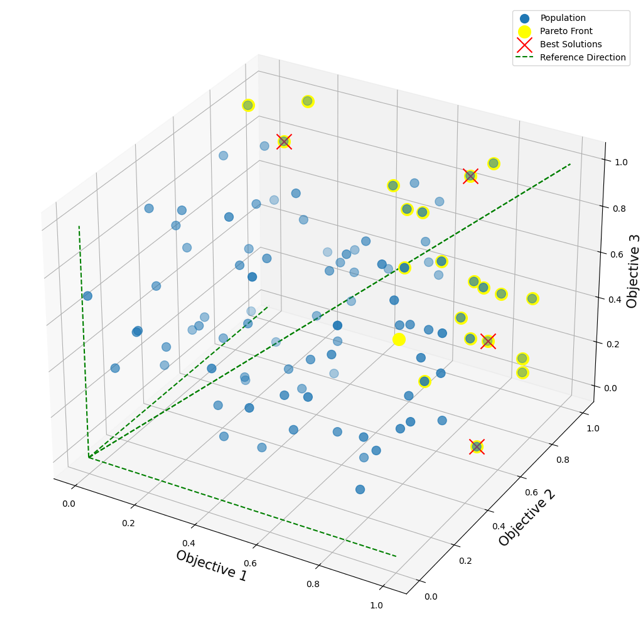
\includegraphics[scale=0.4]{NSGA3.png}
            \caption{Example of Selection using Pareto Optimization and NSGA-\uppercase\expandafter{\romannumeral3}.}
            \label{nsga3}
        \end{figure}


        % 일반적인 GP의 \textit{selection}은 $P$에서 $pop\_size/2$ 만큼 짝을 짓습니다. 이는 일반적으로 GP가 우수한 해 1개를 찾는 것을 목표로 하기 때문입니다. 하지만 우리의 경우 모든 $P_{W}$에 대해 solution을 만드는 것을 목표로 합니다. 그렇기 때문에 $P_{W}$의 양만큼 $p_{w}$와 $p_{r}$의 쌍을 선택합니다. 우리의 \textit{selection} 방법은 elite selection\footnote{\textbf{Elite selection}은 자주 사용하는 진화 전략 중 하나로, 전체 인구 중 상위 일부를 선택하여 그대로 복사하는 방식으로 진행됩니다. 이를 통해 최적의 솔루션을 더 빨리 찾을 수 있습니다.}및 NSGA-\uppercase\expandafter{\romannumeral3} (Non-dominated Sorting Genetic Algorithm) \cite{blank2019investigating}를 사용합니다. Algorithm \ref{alg:MENTORED}의 line 12에 의해 $P$는 무한히 커질 수 있기 때문에 search space를 줄이기 위해서 우수한 해들을 sampling 할 필요가 있습니다. 그래서 우리는 elite selection을 통해 우수한 해인 $P_{C}$와 $S$에 속한 programs를 $pop\_size$ 만큼 sampling 합니다. 만약 $P_{C}$와 $S$가 없다면 $P$에서 $pop\_size$ 만큼 random selection 을 수행합니다. 그 다음, \textit{Fitness Evaluation} (Section \ref{fitness})을 통해 samples의 점수를 계산합니다. 그리고 점수를 기반으로 NSGA-\uppercase\expandafter{\romannumeral3} 알고리즘을 통해 samples 중 최적의 해인 $p_{r}$를 선택합니다. Fig. \ref{nsga3}는 \textsc{Mentored}의 NSGA-\uppercase\expandafter{\romannumeral3}를 이용한 \textit{selection} 방법의 예시를 보여줍니다. $fitness\;funtion$을 통해 0$\sim$1까지 normalized 된 three objectives에 대해 각 samples의 score를 계산합니다. 그 다음, 각각의 objective에 대해 pareto front에 있는 sample 만을 선택합니다. 왜냐하면 여러 objective functions가 있을 때, 하나의 해가 모든 objective functions에서 동시에 최적이 되는 것이 불가능할 때가 많기 때문입니다. 이러한 경우, 여러 objective functions 간의 trade-off을 고려하여 최적 해들을 찾게 되는데, 이때 사용되는 개념이 pareto front입니다. 즉, pareto front로 각각의 objective에 대해 maximum 값을 갖는 우수한 samples로 한 번더 선택의 폭을 좁힙니다. 이후 NSGA-\uppercase\expandafter{\romannumeral3}에서는 $n$개의 reference directions을 만들고 reference directions과 가장 가까운 해를 선택합니다. Fig. \ref{nsga3}의 경우, [1,1,1], [0,0,1], [0,1,0], [1,0,0]로 모든 objective에 대해 우수한 reference direction 1개와 각각의 objective에서만 우수한 reference directions 3개로 총 4개를 만듭니다. 그리고 각각의 reference direction에 대해 가장 가까운 해를 선택합니다. 그럼 결과적으로 4개의 해가 선택되고 random selection을 통해 $p_{r}$를 선택하여 $p_{w}$과 짝을 짓습니다.
        In general GP, \textit{selection} pairs up to $pop\_size/2$ from $P$, as the goal is typically to find a single optimal solution. However, in our case, the goal is to generate solutions for every $P_{W}$. Therefore, we set $pop\_size$ to $|P_{W}|$ and select pairs of $p_{w}$ and $p_{r}$ up to $pop\_size$. Our \textit{selection} method uses elite selection\footnote{\textbf{Elite selection} is one of the commonly used evolutionary strategies where the top individuals from the population are selected and copied as they are, helping to find optimal solutions faster.} and NSGA-\uppercase\expandafter{\romannumeral3} (Non-dominated Sorting Genetic Algorithm) \cite{blank2019investigating}. Since $P$ can grow infinitely, as mentioned in line 12 of Algorithm \ref{alg:MENTORED}, we need to sample the best solutions to reduce the search space. Thus, through elite selection, we sample programs up to $pop\_size$ from $P_{C}$ and $S$. If $P_{C}$ and $S$ does not exist, we samples from $P_{W}$. Then, using \textit{Fitness Evaluation} (Section \ref{fitness}), we calculate the scores of the samples. Based on these scores, NSGA-\uppercase\expandafter{\romannumeral3} selects the optimal solution $p_{r}$ for $p_{w}$ from the samples. Fig. \ref{nsga3} illustrates an example of the \textit{selection} method using NSGA-\uppercase\expandafter{\romannumeral3} in \textsc{Mentored}. For three objectives normalized to 0-1, the fitness function calculates the scores of each sample. Then, only the samples on the pareto set for each objective are selected. This is because, when there are multiple objective functions, it is often impossible for a single solution to be optimal across all objectives simultaneously. In such cases, the pareto optimization is used to find optimal solutions by considering the trade-offs between objectives. In this way, the selection is further narrowed to the best samples for each objective through the pareto set. NSGA-\uppercase\expandafter{\romannumeral3} then generates reference directions and selects the solutions closest to these reference directions. In Fig. \ref{nsga3}, has four reference directions: one that is optimal across all objectives $[1,1,1]$, and three that are optimal for each objective $[0,0,1]$, $[0,1,0]$, $[1,0,0]$. At least four solutions closest to each reference direction are selected, and one $p_{r}$ is finally selected through random selection and paired with $p_{w}$.


    \subsection{Switch Variables}\label{swtVariable}
        % 학생들의 프로그램은 각기 다른 변수명으로 작성될 수 있습니다. 그래서 패치를 생성하기 전에 $p_{w}$과 $p_{r}$의 변수명을 통일시켜야 합니다. 두 프로그램의 변수명을 통일 시키기 위해서 우리는 4가지의 전략을 통해 변수명을 매핑합니다. 첫 번째, Dynamic Equivalence Analysis (DEA) \cite{hu2019re}에서는 $T$를 통해 두 프로그램을 실행하면서 모든 변수의 variable value sequence (VVS)를 수집합니다. 이때, 두 프로그램간에 VVS가 동일한 변수가 있다면 동등한 변수로 매핑합니다. 두 번째, DEA에서 매핑되지 못한 변수들의 VVS를 가지고 Longest Common Sequence (LCS)를 계산합니다. 그래서 가장 많은 LCS의 변수들끼리 매핑합니다. 세 번째, 변수의 type 매칭을 통해 두 프로그램의 변수를 매핑합니다. type matching은 변수의 value는 확인하지 않고 오직 type만을 비교합니다. 마지막 네 번째는 변수명이 동일한 변수들끼리 매핑합니다. 앞서 말했듯 $p_{w}$이 wrong program으로 select 되고 $p_{r}$는 $p_{w}$을 수정하기 위한 reference program으로 select 되었습니다. 그래서 매핑된 변수를 가지고 $p_{r}$의 변수명을 $p_{w}$의 변수명으로 switch 하여 두 프로그램의 변수명을 통일시켜 줍니다.
        Students' programs can be written with different variable names. Therefore, before generating patches, the variable names of $p_{w}$ and $p_{r}$ must be unified. To unify the variable names of the two programs, we map the variable names through four strategies. First, in Dynamic Equivalence Analysis (DEA) \cite{hu2019re}, run both programs using $T$ and collect the Variable Value Sequences (VVS) of all variables. If there are variables with the same VVS between the two programs, map them as equivalent variables. Second, for the variables that were not mapped by DEA, calculate the Longest Common Sequence (LCS) of their VVS and use it for map the leftover variables. Third, map the variables of the two programs through type matching. In type matching, we only compare their types not values. Lastly, the fourth strategy maps variables with the same names. As previously mentioned, $p_{w}$ is selected as the wrong program and $p_{r}$ is selected as the reference program to repair $p_{w}$. Therefore, switch the variable names of $p_{r}$ to the those of $p_{w}$ with the mapped variables to unify the variable names of both programs.


    \subsection{Fault Localization}\label{faultLocalization}
        % 대부분의 AFG approaches \cite{singh2013automated, d2016qlose, gulwani2018automated, wang2018search, hu2019re}은 correct program과 syntactically or semantically different 한 부분을 wrong program의 결함 위치를 식별합니다. 이러한 방식은 correct program 이 다양하지 않거나 wrong program 과 구조적으로 많이 다를 경우 결함이 아닌 부분도 결함으로 식별할 수 있습니다. 그래서 우리는 test cases를 이용한 Fault Localization (FL) 방법을 사용합니다. FL 방법 중 가장 대중적인 Spectrum-Based Fault Localization (SBFL) \cite{abreu2009spectrum}은 프로그램의 실행 스펙트럼을 분석하여 오류가 발생할 가능성이 높은 코드 부분을 식별합니다. 각 코드 요소의 실행 빈도와 테스트 케이스의 성공/실패 결과를 기반으로 의심스러운 정도를 계산합니다. 대표적인 예로는 Tarantula \cite{jones2001visualization}와 Ochiai \cite{abreu2006evaluation} 기법이 있습니다. 하지만, 기존의 FL 방법들은 APR과 마찬가지로 주로 전문가 프로그램을 대상으로 개발되었습니다. 그러다 보니 test cases가 많지 않고 코드가 짧은 학생 프로그램에서는 결함을 잘 식별하지 못합니다. 특히, 학생들의 코드는 분기점이 별로 없다보니 같은 블록의 모든 라인에 대해 동일한 의심도를 부여하곤 합니다. VsusFL \cite{li2023vsusfl} 은 이러한 학생 프로그램에서의 결함 위치 식별 문제를 해결하기 위해 제안되었습니다. VsusFL은 wrong program의 VVS를 수집하여 가장 유사한 VVS를 갖는 correct program을 찾습니다. 그 다음, correct program과 다른 VVS를 갖는 wrong program의 라인을 결함 위치로 식별하여 의심도를 계산합니다. 우리는 \textit{selection} 과정에서 짝지은 $p_{r}$를 $p_{w}$에 대한 correct program이라 가정하고 VsusFL을 사용하여 $p_{w}$에 대한 라인별 의심도를 계산합니다.
        Most AFG approaches \cite{singh2013automated, d2016qlose, gulwani2018automated, wang2018search, hu2019re} identify the fault location of the wrong program by comparing it with syntactically or semantically different parts of the correct program. This method can identify non-fault locations as faults when the correct program is not diverse, or structurally different from the wrong program. To address this problem, we use a Fault Localization (FL) method based on test cases. Among FL methods, the most popular one is Spectrum-Based Fault Localization (SBFL) \cite{abreu2009spectrum}, which analyzes the execution spectrum of a program to identify statements that are most likely to contain faults. It calculates the suspiciousness ($susp$) of statements based on the execution frequency and the success/failure results of the test cases. Representative techniques include Tarantula \cite{jones2001visualization} and Ochiai \cite{abreu2006evaluation}. However, traditional FL methods were mainly developed for expert-level programs such as APR. As a result, they struggle to effectively identify faults in student programs, which tend to have fewer test cases and shorter code. Specifically, since student code often has fewer branching points, these methods tend to assign the same level of $susp$ to all statements within a block. VsusFL \cite{li2023vsusfl} was proposed to address this issue in student programs. VsusFL collects the VVS of the wrong program and finds the correct program with the most similar VVS. Then, it identifies the statements of the wrong program with different VVS from the correct program as fault locations and calculates the $susp$. In our approach, we set the $p_{r}$ selected during the \textit{selection} phase to be the correct program for $p_{w}$ and use VsusFL to calculate the $susp$ of statements for $p_{w}$.


    \subsection{Program Repair}\label{programRepair}

        % \RestyleAlgo{ruled}
        % \SetKwComment{Comment}{/*}{*/}
        % \begin{algorithm}[hbt!]
        %     \caption{programRepair} \label{alg:programRepair}
        %     \SetKwInOut{Input}{Input}
        %     \Input{$p_{w} - Wrong\;program$\\$p_{r} - Reference\;program$\\$susp - Suspiciousness\;of\;faults$\\$T - Set\;of\;test\;cases$\\$H - History\;of\;fixes$}
        %     \KwOut{$p_{f} - Fixed\;program$}
        %     \hrulealg
        %     $N \gets nodeMap(p_{w}, p_{r}, T)$\;
        %     \SetKwRepeat{Repeat}{repeat}{until}
        %     \Repeat{$N = \varnothing$}
        %     {
        %         $N_{cut} \gets crossoverMap(N)$\;
        %         $N_{mut} \gets mutationMap(N, susp)$\;
        %         $N_{fix} \gets N_{cut}\;\bigcup\;N_{mut}$\;
        %         $p_{f} \gets fixer(p_{w}, N_{fix})$\;
        %         \eIf{$\langle p_{w}, p_{f} \rangle \notin H$}{
        %             $H \gets H\;\bigcup\;\langle p_{w}, p_{f} \rangle$\;
        %             \Return $p_{f}$\;
        %         }{
        %             $N \gets N - N_{fix}$\;
        %         }
        %     }
        %     \Return $None$\;
        % \end{algorithm}

        % wrong program을 수정하기 위해선 결함에 따른 패치가 필요합니다. 그래서 우리는 $p_{w}$의 결함에 대한 패치를 $p_{r}$에서 찾기 위해 프로그램의 execution traces 정보를 활용합니다. 결함과 패치를 매핑하기 앞서 우리는 프로그램의 node 기반으로 수정을 하기 때문에 먼저, 두 프로그램을 Abstract Syntax Tree (AST)로 represent 합니다. 그 다음, \textit{replace}, \textit{insert}, \textit{delete}의 3가지 방법에 따라 두 프로그램의 노드들을 매핑합니다. node mapping은 프로그램의 execution trace을 기반으로 하며, test cases $T$를 통해 각 프로그램의 실행 경로를 추출합니다. 이 과정에서 각 프로그램의 line number가 서로 일치하지 않을 수 있기 때문에, 각 line을 구성하는 statement의 reserved word에 해당하는 노드로 대체하여 처리합니다. 먼저 \textit{replace}를 위한 node mapping은 LCS을 이용하여 매핑합니다. 그 다음, \textit{insert}를 위한 node mapping은 \textit{replace} 과정에서 매핑되지 않은 $p_{r}$의 노드들을 매핑합니다. 단, \textit{insert}는 추가적으로 어느 위치에 insert 될지를 정해야 합니다. 그래서 우리는 \textit{replace}에서 매핑된 노드들을 기준으로 \textit{insert} node와 depth가 같은 노드가 있으면 해당 노드의 형제 노드로 insert 되고 depth가 같은 노드가 없으면 child 노드로 insert 합니다. 마지막 \textit{delete}를 위한 node mapping은 \textit{replace}에서 매핑되지 않은 $p_{w}$의 노드들을 매핑하는데 delete 하는것이기 때문에 None으로 매핑합니다. 매핑된 노드들은 $p_{w}$의 faults와 $p_{r}$의 patches 연결짓는데 사용됩니다. 기존 AFG approaches 들의 Control Flow Structure (CFS)를 기반으로 매핑하는 방법은 두 프로그램의 CFS가 일치해야 한다는 한계가 있습니다. 하지만 우리의 node mapping는 execution trace를 기반으로 하다 보니 CFS에 제한적이지 않습니다.
        To repair the wrong program, patches corresponding to the faults are required. Therefore, we utilize execution traces of the program to find patches for the faults in $p_{w}$ from $p_{r}$. Before mapping the faults and patches, we first represent the two programs as Abstract Syntax Trees (AST) since we repair the program based on the nodes. Next, we map the nodes of the two programs according to the three methods of \textit{replace}, \textit{insert}, and \textit{delete}. The node mapping is based on the execution traces of the program, and extracts the execution paths of each program using $T$. In this process, the line numbers of each program may not same, so we replace each line of execution paths with the nodes corresponding to the reserved words of the statement that makes up the line. First, the node mapping for \textit{replace} is mapped using the LCS. Next, the node mapping for \textit{insert} maps the nodes of $p_{r}$ that were not mapped in the \textit{replace} map. However, \textit{insert} must also determine where to insert. Therefore, we insert the node as a sibling node if there is a node with the same depth as the \textit{insert} node among the mapped nodes from \textit{replace}, and as a child node if there is no node with the same depth. Finally, the node mapping for \textit{delete} maps the nodes of $p_{w}$ that were not mapped in the \textit{replace} map as None, as they are to be deleted. The mapped nodes are used to connect the faults of $p_{w}$ with the patches of $p_{r}$. The mapping method of existing AFG approaches \cite{gulwani2018automated, wang2018search,hu2019re} based on the Control Flow Structure (CFS) has the limitation that the CFS of the two programs must match. However, our node mapping is not limited by the CFS as it is based on the execution traces.
        
        \begin{figure}[h]
            \centering
            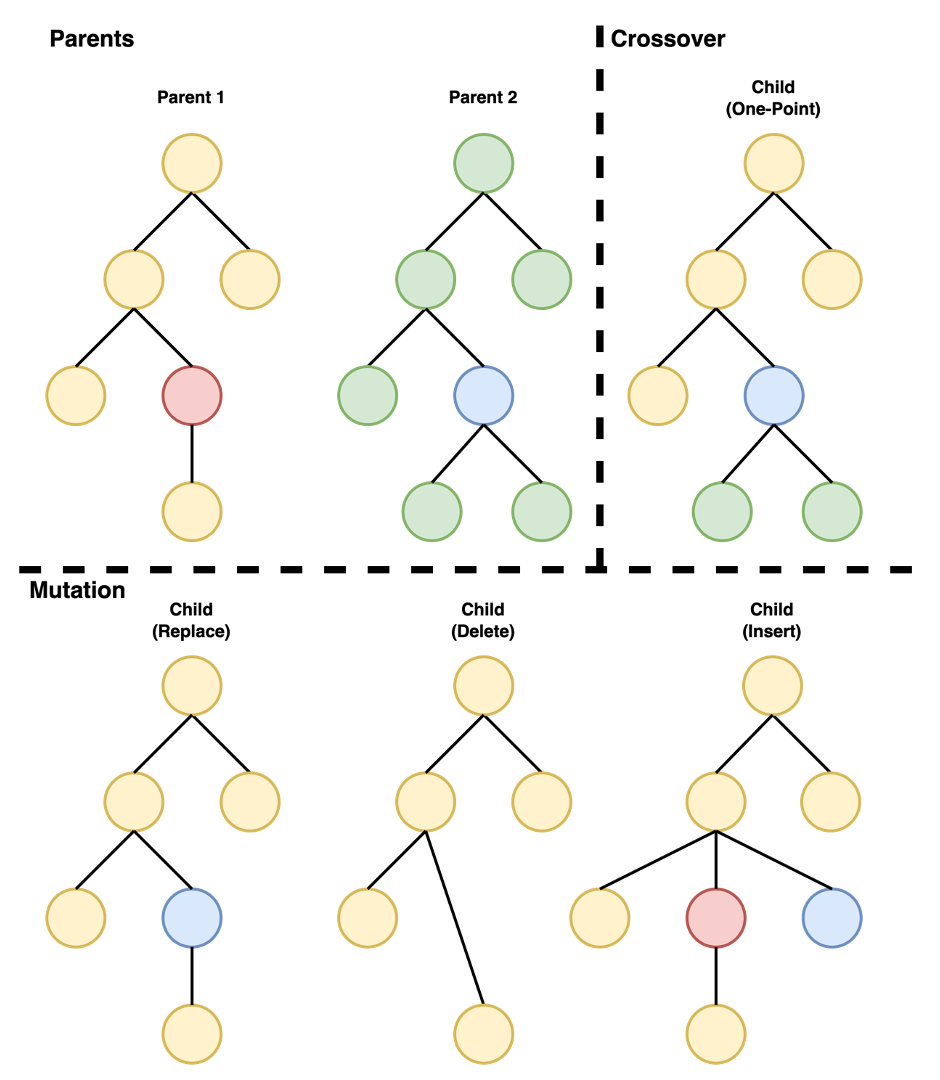
\includegraphics[scale=0.4]{repair.png}
            \caption{Genetic operators for AST}
            \label{fig:repair}
        \end{figure}

        % GP는 일반적으로 crossover와 mutation을 사용합니다. crossover는 GP에서 두 부모 프로그램의 일부 코드 조각을 교환하여 새로운 자식 프로그램을 생성하는데 사용되는 진화 연산입니다. 이는 생물학에서 유전자가 교차되는 현상을 모델링한 것으로, GP에서는 프로그램의 효율성과 다양성을 높이기 위해 사용됩니다. 그리고 mutation은 프로그램의 코드에 임의의 변화를 도입하여 프로그램의 동작이나 구조를 변형시키는 진화 연산입니다. 이 과정은 유전 알고리즘에서의 다양성을 증진시키고 local optima에 빠지는 것을 방지하는 데 중요한 역할을 합니다. 따라서 우리의 수정 또한 crossover와 mutation을 사용합니다. 먼저, crossover를 위해서는 cut point를 선택해야합니다. 그래서 우리는 \textit{replace}에서 매핑된 노드들 중 하나를 random 하게 선택하여 \textit{one-point-crossover}를 통해 $p_{w}$를 수정합니다. 그 다음, 우리는 \textit{replace}, \textit{insert}, \textit{delete}의 3가지 edit action에 의해 mutation을 수행합니다. mutation은 $susp$의 의심도를 기반으로 mutation 할 위치를 선택합니다. 이는 \textit{replace}, \textit{insert}, \textit{delete}에서 매핑된 노드들 중 $susp$를 기반으로 roulette wheel selection \cite{eiben2015introduction}을 진행하여 하나를 random 하게 선택하여 $p_{w}$를 수정합니다. Fig \ref{fig:repair}은 crossover와 mutation을 통한 수정 방법을 보여줍니다. Parent1 $p_{w}$과 Parent2 $p_{r}$는 AST로 represent한 것입니다. $p_{w}$의 빨간색 노드가 결함이고 $p_{r}$의 파란색 노드가 패치라고 할 때, crossover의 \textit{one-point-crossover}는 결함 노드(red)를 포함한 모든 하위 노드를 패치 노드(blue)와 모든 하위 노드로 교환합니다. mutation의 \textit{replace}는 결함 노드를 패치 노드로 대체합니다. \textit{delete}는 결함 노드를 삭제하는데 결함 노드 하위에 노드가 있을 경우 결함 노드의 부모 노드와 자식 노드를 연결합니다. \textit{insert}는 결함 노드를 기준으로 봤을 때, 형제 노드에 해당하므로 결함 노드의 다음 형제 노드로 삽입합니다. crossover는 기준 되는 노드의 하위 노드들이 모두 수정되지만 mutation은 기준 노드끼리만 수정됩니다. 이러한 수정 방법을 통해 $p_{w}$의 결함을 수정하여 $p_{f}$를 생성합니다.
        Genetic Programming (GP) typically uses crossover and mutation to create new child programs. Crossover is an evolutionary operation used in GP to exchange parts of the code of two-parent programs. It models the phenomenon of gene crossover in biology and increase the efficiency and diversity of programs. On the other hand, Mutation introduces random changes to the code of a program to alter its behavior or structure. It also models the phenomenon of gene mutation in biology and increase diversity of programs and preventing them from falling into local optima. Therefore, we also use crossover and mutation for our repair process. First, to perform crossover, we use \textit{one-point-crossover} to repair $p_{w}$. Thus, we randomly select one of the nodes mapped in \textit{replace} as a cut point and exchange the node of $p_{w}$ with the node of $p_{f}$. Next, we perform mutation based on the three edit actions of \textit{replace}, \textit{insert}, and \textit{delete}. Mutation selects the location to mutate based on the $susp$. This is done by performing roulette wheel selection \cite{eiben2015introduction} on the nodes mapped in \textit{replace}, \textit{insert}, and \textit{delete} as mutation point, and applying the selected action and node. Fig \ref{fig:repair} shows the repair process through crossover and mutation. Assuming $Parent1$ is $p_{w}$ and $Parent2$ is $p_{r}$. The red node of $Parent1$ are faults, and the blue node of $Parent2$ are patches. In crossover, \textit{one-point-crossover} exchanges fault node (red) and its children with patch node (blue) and its children. In mutation, \textit{replace} replaces the fault node with the patch node. \textit{delete} deletes the fault node, if there are nodes below the fault node it connects the parent node and child node of the fault node. \textit{insert} inserts the fault node as the next sibling node of the fault node if two nodes have the same depth otherwise, it inserts to children. In crossover, the patch node and all of its children are repaired, but in mutation, only the patch node are repaired. Through these repair methods, the faults in $p_{w}$ are repaired to generate $p_{f}$.



    \subsection{Fitness Evaluation}\label{fitness}
        % Fitness evaluation을 통해 프로그램이 주어진 문제를 얼마나 잘 해결하는지를 평가합니다. 이 함수는 GP의 핵심 요소 중 하나로, 개별 프로그램의 성능을 측정하고 이를 바탕으로 향후 세대에서 선택될 개체를 결정합니다. Fitness evaluation은 \textit{selection} (Section \ref{Selection}) 과정에서 $p_{w}$의 짝인 $p_{r}$을 선택할 때, 그리고 Algorithm \ref{alg:MENTORED}의 line 12에서 우수한 프로그램을 향후 세대에서 사용될 수 있도록 population $P$에 추가하는데 사용됩니다. 우리는 총 4가지의 objective functions를 설정하여 프로그램의 성능을 측정합니다. 참고로 모든 objective functions는 $p_{w}$을 기준으로 상대적인 프로그램의 성능을 측정합니다. 또한, 모든 objective functions는 0$\sim$1 사이의 값을 가지며 1에 가까울수록 높은 적합도를 갖습니다. The four objective functions are formulated as follows:
        Fitness evaluation is used to evaluate how well the program solves a given problem. Fitness evaluation is one of the core elements of GP, as it calculates the performance of individual programs and determines which candidates will be selected for future generations. we use it in the \textit{selection} process (Section \ref{Selection}) when selecting $p_{r}$, the pair of $p_{w}$, and in line 12 of Algorithm \ref{alg:MENTORED}, where the best-performing programs are added to the population $P$ for future generations. We define four objective functions to calculate the performance of programs. All objective functions evaluate the performance of programs relative to $p_{w}$. Additionally, all objective functions have values between 0 and 1, where values closer to 1 indicate higher fitness. The four objective functions are formulated as follows:

        \begin{equation}
            f_{1}(\mathbf{p'})=\frac{|\left\{t\in T_{F}|\;\mathbf{p'}\;passes\;t\right\}|}{|T_{F}|} 
        \end{equation}
        \begin{equation}
            f_{2}(\mathbf{p'})=\frac{|\left\{t\in T_{P}|\;\mathbf{p'}\;passes\;t\right\}|}{|T_{P}|} 
        \end{equation}
        \begin{equation}
            f_{3}(\mathbf{p'})=\frac{\sum_{\substack{t \in T_{F \veryshortrightarrow P}}} E_{sim}(\mathbf{p'}, t)}{|T_{F \veryshortrightarrow P}|}
        \end{equation}
        \begin{equation}
            f_{4}(\mathbf{p'})=\frac{\sum_{\substack{t \in T_{P \veryshortrightarrow P}}} E_{sim}(\mathbf{p'}, t)}{|T_{P \veryshortrightarrow P}|}
        \end{equation}

        % $f_{1}(\mathbf{p'})$는 $p_{w}$이 실패한 test cases를 반대로 passes한 test cases를 계산한 objective function입니다. $T_{F}$는 $p_{w}$이 실패한 test cases를 의미합니다. $f_{2}(\mathbf{p'})$는 $p_{w}$이 통과한 test cases를 똑같이 passes한 test cases를 계산한 objective function입니다. $T_{P}$는 $p_{w}$이 통과한 test cases를 의미합니다. $f_{3}(\mathbf{p'})$는 $p_{w}$은 실패하고 $p$는 통과한 test cases로 execution traces 기반 유사도를 계산한 objective function입니다. $T_{F \veryshortrightarrow P}$는 $p_{w}$은 실패하고 $p$는 통과한 test cases를 의미합니다. $f_{4}(\mathbf{p'})$는 $p_{w}$과 $p$ 모두 통과한 test cases로 execution traces 기반 유사도를 계산한 objective function입니다. $T_{P \veryshortrightarrow P}$는 $p_{w}$이 통과하고 $p$도 똑같이 통과한 test cases를 의미합니다. $E_{sim}(\mathbf{p'}, t)$는 두 프로그램의 execution traces 기반 유사도를 의미합니다. execution traces 기반 유사도는 $p_{w}$과 $p'$의 execution traces $E_{trace}$의 LCS를 MAX 개수로 나누어 계산하는것으로 LCS는 program repair 과정(Section \ref{programRepair})의 node mapping 과정에서 매핑된 노드들의 개수와 같습니다. execution traces 기반 유사도의 공식은 다음과 같습니다:
        $f_{1}(\mathbf{p'})$ is an objective function that calculates the number of test cases passed by $p'$ that were failed by $p_{w}$. $T_{F}$ means the test cases that $p_{w}$ failed. $f_{2}(\mathbf{p'})$ is an objective function that calculates the number of test cases passed by $p'$ that were also passed by $p_{w}$. $T_{P}$ means the test cases that $p_{w}$ passed. $f_{3}(\mathbf{p'})$ is an objective function that calculates the similarity based on the execution traces for the test cases that $p_{w}$ failed but $p'$ passed. $T_{F \veryshortrightarrow P}$ means the test cases that $p_{w}$ failed but $p'$ passed. $f_{4}(\mathbf{p'})$ is an objective function that calculates the similarity based on the execution traces for the test cases passed by both $p_{w}$ and $p'$. $T_{P \veryshortrightarrow P}$ means the test cases that were passed by both $p_{w}$ and $p'$. $E_{sim}(\mathbf{p'}, t)$ means the execution traces-based similarity between the two programs. It is calculated by dividing the LCS of the execution traces $E_{trace}$ of $p_{w}$ and $p'$ by the max number of nodes. The LCS corresponds to the number of nodes mapped in the node mapping process during the program repair process (Section \ref{programRepair}). The formula for execution traces-based similarity is as follows:


        \begin{equation}
            E_{sim}(\mathbf{p'}, t)=\frac{LCS(E_{trace}(p_{w}, t), E_{trace}(\mathbf{p'}, t))}{MAX(E_{trace}(p_{w}, t), E_{trace}(\mathbf{p'}, t))}
        \end{equation}

        % 각각의 objective function에 대해 어떤것이 우수 하고 열등한지 정하는것은 매우 어려운 작업입니다. 그래서 우리는 각각의 objective function에 대한 가중치 대신 NSGA-\uppercase\expandafter{\romannumeral3}를 통해 프로그램의 적합도를 평가합니다. 이러한 방식은 다수의 objective functions를 처리하는데 효과적이며 해의 다양성을 보장하기 때문에 다양한 수정이 가능하게 합니다.
        Determining which objective function is superior or inferior for each case is challenging. Therefore, instead of assigning weights to each objective function, we evaluate the fitness of programs using NSGA-\uppercase\expandafter{\romannumeral3}. This method effectively handles multiple objective functions and ensures diverse solutions, allowing for various modifications.

\begin{table*}[hb!]
    \centering
    \captionof{table}{Results of AFG approaches on 15 programming assignments}
    \label{tab:tab1}
    \resizebox{\textwidth}{!}{
        \begin{tabular}{ |c|c|c|c|ccc|ccc|ccc| } 
            \hline
            \multirow{3}{*}{NO} & \multirow{3}{*}{Title} & \multirow{3}{*}{\makecell[l]{\#Correct \\ Programs}} & \multirow{3}{*}{\makecell[l]{\#Wrong \\ Programs}} & \multicolumn{9}{c|}{$W/\;\chi\;\;(W/O\;\chi)$} \\
            \cline{5-13}
            & & & & \multicolumn{3}{c|}{Repair Rate ($RR$)} & \multicolumn{3}{c|}{Relative Patch Size ($RPS$)} & \multicolumn{3}{c|}{Average Time Taken ($ATT$/sec)} \\
            \cline{5-7} \cline{8-10} \cline{11-13}
            & & & & \textsc{Refactory} & \textsc{PyDex} & \textsc{Mentored} & \textsc{Refactory} & \textsc{PyDex} & \textsc{Mentored} & \textsc{Refactory} & \textsc{PyDex} & \textsc{Mentored} \\
            \hline\hline
            1 & Theatre Square & 30 & 20 & 
            0.45 (0.95) & \textbf{1.00} (\textbf{1.00}) & \textbf{1.00} (0.60) & 
            0.51 (0.97) & \textbf{0.26} (\textbf{0.25}) & 0.33 (0.90) & 
            2.6 (3.3) & 0.5 (1.5)+240 & \textbf{1.8} (\textbf{1.8}) \\
            \hline
            2 & Watermelon & 14 & 31 & 
            0.97 (0.19)& 0.97 (0.26) & \textbf{1.00} (\textbf{1.00}) & 
            0.54 (0.90) & 0.50 (\textbf{0.19}) & \textbf{0.26} (0.28) & 
            0.4 (3.0) & 0.4 (1.2)+240 & \textbf{0.3} (\textbf{0.3}) \\
            \hline
            3 & Domino Piling & 40 & 10 & 
            0.80 (0.00)& 0.80 (\textbf{0.80}) & \textbf{1.00} (\textbf{0.80}) & 
            0.26 (nan) & \textbf{0.07} (\textbf{0.07}) & 0.21 (0.66) & 
            \textbf{0.3} (3.3) & 0.5 (1.5)+240 & 0.6 (\textbf{0.5}) \\
            \hline
            4 & Petya and Strings & 38 & 13 & 
            0.92 (0.77)& \textbf{1.00} (\textbf{0.85}) & \textbf{1.00} (0.62) & 
            0.68 (0.89) & \textbf{0.35} (\textbf{0.20}) & 0.44 (0.29) & 
            12.6 (6.8) & 0.6 (1.6)+240 & \textbf{0.9} (\textbf{0.8}) \\
            \hline
            5 & String Task & 32 & 16 & 
            0.94 (0.94)& \textbf{1.00} (\textbf{1.00}) & \textbf{1.00} (\textbf{1.00}) & 
            0.47 (1.16) & \textbf{0.13} (\textbf{0.15}) & 0.17 (0.17) & 
            5.6 (6.9) & 1.4 (1.5)+240 & \textbf{3.2} (\textbf{1.8}) \\
            \hline
            6 & Next Round & 24 & 25 & 
            \textbf{1.00} (\textbf{1.00})& \textbf{1.00} (0.44) & \textbf{1.00} (\textbf{1.00}) & 
            0.53 (0.77) & 0.37 (\textbf{0.15}) & \textbf{0.35} (0.61) & 
            4.6 (5.4) & 0.8 (1.5)+240 & \textbf{0.7} (\textbf{0.8}) \\
            \hline
            7 & Beautiful Matrix & 42 & 8 & 
            \textbf{1.00} (\textbf{0.88})& \textbf{1.00} (0.75) & \textbf{1.00} (0.12) & 
            0.45 (0.76) & \textbf{0.23} (\textbf{0.03}) & 0.47 (\textbf{0.03}) & 
            1.7 (4.1) & 0.6 (1.4)+240 & \textbf{1.2} (\textbf{0.9}) \\
            \hline
            8 & Stones on the Table & 44 & 9 & 
            0.67 (0.89)& \textbf{1.00} (0.67) & \textbf{1.00} (\textbf{1.00}) & 
            0.49 (0.52) & \textbf{0.31} (\textbf{0.18}) & \textbf{0.31} (0.41) & 
            4.9 (5.5) & 0.8 (1.8)+240 & \textbf{2.4} (\textbf{1.9}) \\
            \hline
            9 & Word Capitalization & 45 & 6 & 
            0.33 (\textbf{1.00})& 0.50 (0.33) & \textbf{1.00} (\textbf{1.00}) & 
            0.72 (1.63) & \textbf{0.56} (\textbf{0.50}) & 0.61 (1.22) & 
            \textbf{0.2} (\textbf{0.2}) & 0.4 (1.2)+240 & 0.4 (0.3) \\
            \hline
            10 & Helpful Maths & 47 & 4 & 
            0.75 (\textbf{1.00})& \textbf{1.00} (\textbf{1.00}) & \textbf{1.00} (0.25) & 
            0.78 (1.87) & \textbf{0.09} (0.24) & 0.45 (\textbf{0.10}) & 
            4.8 (27.0) & 0.8 (1.6)+240 & \textbf{3.9} (\textbf{1.9}) \\
            \hline
            11 & Sequential Search & 768 & 575 & 
            0.98 (0.60)& \textbf{1.00} (0.89) & 0.97 (\textbf{0.98}) & 
            0.39 (0.68) & \textbf{0.29} (\textbf{0.26}) & \textbf{0.29} (0.33) & 
            3.0 (3.3) & 1.8 (2.3)+240 & \textbf{1.7} (\textbf{3.1}) \\
            \hline
            12 & Unique Dates and Months & 291 & 435 & 
            0.79 (0.55)& \textbf{0.90} (\textbf{0.81}) & 0.62 (0.54) & 
            0.46 (0.63) & \textbf{0.25} (\textbf{0.22}) & 0.27 (0.24) & 
            \textbf{2.8} (\textbf{4.1}) & 1.7 (2.0)+240 & 4.7 (7.1) \\
            \hline
            13 & Duplicate Elimination & 546 & 308 & 
            0.97 (0.63)& 0.98 (\textbf{1.00}) & \textbf{1.00} (0.99) & 
            0.33 (0.67) & \textbf{0.31} (\textbf{0.32}) & 0.38 (0.35) & 
            4.5 (3.2) & 1.7 (1.7)+240 & \textbf{2.6} (\textbf{3.1}) \\
            \hline
            14 & Sorting Tuples & 419 & 357 & 
            0.84 (0.62)& \textbf{1.00} (\textbf{0.98}) & 0.97 (0.97) & 
            \textbf{0.26} (1.75) & 0.44 (0.31) & 0.39 (\textbf{0.30}) & 
            6.7 (7.8) & 1.7 (1.7)+240 & \textbf{4.6} (\textbf{4.4}) \\
            \hline
            15 & Top-K & 418 & 108 & 
            0.84 (0.95)& \textbf{1.00} (\textbf{0.99}) & \textbf{1.00} (0.97) & 
            0.29 (0.78) & \textbf{0.22} (\textbf{0.25}) & \textbf{0.22} (0.37) & 
            14.4 (\textbf{4.9}) & 0.8 (1.2)+240 & \textbf{7.9} (6.5) \\
            \hline\hline
            \multicolumn{2}{|c|}{Overall} & 2973 & 1925 & 
            0.82 (0.73) & 0.94 (0.78) & \textbf{\textcolor{blue}{0.97}} (\textbf{\textcolor{blue}{0.80}}) & 
            0.48 (1.00) & \textbf{\textcolor{blue}{0.29}} (\textbf{\textcolor{blue}{0.22}}) & 0.34 (0.41) & 
            4.6 (5.9) & 1.0 (1.6)+240 & \textbf{\textcolor{blue}{2.5}} (\textbf{\textcolor{blue}{2.4}}) \\
            \hline
        \end{tabular}
    }
    \begin{tablenotes}
        \item Results are shown as with correct program $W/\;\chi$ and without correct program(in parentheses) $W/O\;\chi$.
        \item In $W/O\;\chi$, \textsc{Refactory} uses a single correct program by policy. \textsc{PyDex} and \textsc{Mentored} do not use any correct programs.
    \end{tablenotes}
\end{table*}



\section{Experimental Design}
    % 이번 섹션에서는 답변해야 할 연구 질문, 성능 비교를 위한 baseline approaches, 실험 데이터셋, \textsc{Mentored}의 실험을 위한 평가 메트릭 및 parameters을 설명합니다.
    % In this section, we describe the research questions to be answered, baseline approaches for performance comparison, experimental datasets, evaluation metrics, and parameters for \textsc{Mentored} experiments.

    \subsection{Research Questions}
        % AFG 기법들마다 제공하는 피드백의 형태가 다르기 때문에, 우리는 비교 실험을 위해 공통적으로 사용되는 patch만을 feedback으로 다룹니다. \textsc{Mentored}을 평가하기 위해 다음과 같은 연구 질문을 설정하였습니다.
        Since AFG techniques provide different forms of feedback, we treat only patch as feedback for comparison experiments. We set the following research questions to evaluate \textsc{Mentored}.


        \textbf{RQ1. How effectively can \textsc{Mentored} generate feedback with and without correct programs?}
        % 이전 AFG 연구에서 알 수 있듯 correct program이 많을 수록 feedback 생성률이 향상합니다 \cite{li2022generating, heo2023referent}. 이는 반대로 correct program이 없을 때, feedback 생성이 어렵다는 것을 의미합니다. 실제 소규모 프로그래밍 수업의 과제나 online judge의 새로운 문제들의 경우 correct program이 없을 수 있습니다. 그래서 우리는 correct program을 사용할 때와 사용하지 않았을 때 모두 \textsc{Mentored}가 얼마나 효과적으로 feedback을 생성하는지 이전 연구들과 비교합니다.
        Previous AFG approaches demonstrate that having more correct programs available improves the rate of feedback generation \cite{li2022generating, heo2023referent}. In contrast, the absence of correct programs makes it challenging to generate feedback. In real-world situations, such as small-scale programming course assignments or new online judge problems, there may be no correct programs. Therefore, we assess how effectively \textsc{Mentored} generates feedback both with and without correct programs, comparing its performance to previous approaches.

        \textbf{RQ2. How effectively can \textsc{Mentored} generate diverse feedback?}
        % AFG는 correct programs를 활용하여 패치를 생성하기 때문에 correct programs의 다양성이 부족할 경우 각기 다른 구조의 wrong programs에 대해 똑같은 구조의 fixed program이 피드백으로 제공될 수 있습니다. 이는 다양한 알고리즘을 통해 프로그래밍 스킬을 향상시켜야 하는 학생들에게 치명적일 수 있습니다. 이에 우리는 \textsc{Mentored}가 이러한 한계를 극복하고 얼마나 효과적으로 다양한 피드백을 생성하는지 검토합니다.
        Since AFG generates patches using correct programs, a lack of diversity in correct programs can result in feedback providing fixed programs with the same structure for different wrong program structures. This can be detrimental to students who need to improve their programming skills through exposure to diverse algorithms. Therefore, we examine how effectively \textsc{Mentored} overcomes these limitations and generates diverse feedback.


        \textbf{RQ3. How effectively can \textsc{Mentored} generate high-quality feedback?}
        % 피드백의 질은 학생의 학습을 개선하고 오류를 수정하는 데 중요합니다. 그래서 우리는 피드백의 품질을 측정하고 이전 연구들과 비교하여 \textsc{Mentored}가 얼마나 효과적으로 고품질의 피드백을 생성하는지 검토합니다.
        The quality of feedback is important for improving student learning and repairing faults. Therefore, we measure the quality of feedback and compare it with previous approaches to review how effectively \textsc{Mentored} generates high-quality feedback.


    \subsection{Baselines}
        % \textsc{Mentored}가 얼마나 효과적으로 피드백을 생성하는지 검토하기 위해 공개된 SOTA AFG 기술들을 선택하였습니다. \textsc{Refactory} \cite{hu2019re}는 내가 아는한 공개적으로 사용 가능한 데이터 세트와 tool을 모두 갖춘 가장 최근의 제안방법입니다. \textsc{AssignmentMender} \cite{li2022generating}은 공개된 데이터셋과 논문에서 소개한 데이터셋의 수가 일치하지 않고 tool이 실행불가능했기 때문에 제외합니다. \textsc{PyDex} \cite{zhang2024pydex}은 tool이 공개되어 있진 않지만 LLM을 기반으로 구현되었으며 prompt가 저자의 논문에 공개되어 있기 때문에 직접 구현하여 실험했습니다. Tools for \textsc{Mentored} and \textsc{PyDex} are available in the section \ref{tool}.
        To evaluate how effectively \textsc{Mentored} generates feedback, we selected publicly available state-of-the-art AFG techniques. \textsc{Refactory} \cite{hu2019re} is the most recent publicly available approach with both datasets and tools, to the best of our knowledge. \textsc{AssignmentMender} \cite{li2022generating} was excluded due to discrepancies between the publicly available dataset and the dataset mentioned in the paper, as well as the tool being non-executable. \textsc{PyDex} \cite{zhang2024pydex} is not publicly available as a tool, but since it is based on LLM and the prompt was made publicly available in the author's paper, we implemented it ourselves for the experiments. Tools for \textsc{Mentored} and \textsc{PyDex} are available in Section \ref{tool}.


    \subsection{Datasets}
        % 우리는 우리의 접근 방식을 비교하기 위해 가장 최근의 피드백 생성 접근 방식 중 데이터셋이 공개된 \textsc{Refactory} \cite{hu2019re}와 \textsc{AssignmentMender} \cite{li2022generating}를 선택합니다. \textsc{Refactory}의 dataset은 실제 \textsc{Refactory} 저자의 대학교에서 수집한 파이썬 프로그래밍 기초 강의의 programming assignments로 총 5개의 과제에서 수집하였으며 2442개의 correct programs과 1783개의 wrong programs으로 구성되어 있습니다. 그리고 \textsc{AssignmentMender}의 dataset은 online judge 사이트인 CodeForces\footnote{\url{https://codeforces.com}}에서 가장 인기있는 10개의 programming problems를 수집하였으며 372개의 correct programs와 128개의 wrong programs로 구성되어 있습니다. 하지만 \textsc{AssignmentMender}의 공개된 dataset \cite{ExperimentTask}를 보면 논문에 기재된 것과 달리 320개의 correct programs와 142개의 wrong programs가 존재하였습니다. 그래서 우리는 공개된 dataset을 기준으로 평가하였습니다. 결과적으로 총 15개의 프로그래밍 과제에서 2973개의 correct programs과 1925개의 wrong programs을 datasets으로 실험합니다.
        To compare our approach, we selected two of the most recent feedback generation approaches with publicly available datasets, \textsc{Refactory} \cite{hu2019re} and \textsc{AssignmentMender} \cite{li2022generating}. Dataset from \textsc{Refactory} consists of programming assignments from a Python programming introductory course at the author's university, collected from 5 assignments, including 2,442 correct programs and 1,783 wrong programs. Dataset from \textsc{AssignmentMender} was collected from the 10 most popular programming problems on the online judge site CodeForces\footnote{\url{https://codeforces.com}}, consisting of 372 correct programs and 128 wrong programs. However, upon reviewing dataset of \textsc{AssignmentMender} \cite{ExperimentTask}, we found 320 correct programs and 142 wrong programs, differing from the numbers reported in the paper. Therefore, we conducted our evaluation based on the publicly available dataset. As a result, we experimented with a total of 15 programming assignments, consisting of 2,973 correct programs and 1,925 wrong programs.


    \subsection{Evaluation Metrics}
        % 우리는 AFG의 성능을 평가하기 위해 기존 연구들에서 공통적으로 가장 많이 사용되는 3가지 평가 메트릭을 사용합니다. 첫번째, Repair Rate (RR)는 수리된 wrong program의 비율을 의미합니다. $RR$의 $P_{W}$는 wrong programs를 의미하고 $S$는 $P_{W}$에 대한 solutions를 의미합니다. 두번째, Relative Patch Size (RPS)는 wrong program를 기준으로 fixed program과의 edit distance를 의미합니다. $TED$는 tree edit distance를 의미하고 $AST$는 Abstract Syntax Tree, $p_{w}$는 wrong program, $p_{f}$는 fixed program을 의미합니다. 마지막 세번째, Average Time Taken (ATT)는 한개의 wrong program을 수정하는데 걸린 평균 시간(sec)을 의미합니다. 3가지 평가 메트릭에 대한 공식은 다음과 같습니다:
        To evaluate the performance of AFG, we use three evaluation metrics that are most commonly used in previous studies. First, Repair Rate ($RR$) represents the rate of fixed wrong programs. In $RR$, $P_{W}$ means the wrong programs, and $S$ means the solutions for $P_{W}$. Second, Relative Patch Size ($RPS$) calculates $TED$ between the fixed program ($p_{f}$) and the wrong program ($p_{w}$). Lastly, Average Time Taken ($ATT$) means the average time (in seconds) taken to repair single wrong program. The formulas for these three evaluation metrics are as follows:

        \begin{equation}
            RR = \frac{|S|}{|P_{W}|} \nonumber
        \end{equation}
        \begin{equation}
            RPS = \frac{TED(AST_{w}, AST_{f})}{Size(AST_{w})} \nonumber
        \end{equation}
        \begin{equation}
            ATT = \frac{time\;taken\;of\;approach}{|P_{W}|} \nonumber
        \end{equation}


    \subsection{Parameters}
        % 실험을 하기 앞서 우리의 제안 방법인 \textsc{Mentored}의 글로벌 매개변수를 보고합니다. \textsc{Mentored}는 GP을 기반으로 하기 세대 수를 설정하지 않으면 무한반복 될 수 있습니다. 또한, 무작위성에 따라 결과가 달라질 수 있습니다. 그래서 우리는 세대 반복의 최대 횟수 $N$를 30회로 제한하고 GP에 의해 생성된 childs로 인해 population이 무한 증식하여 search space가 커지는 것을 방지하기 위해 maximum population size $pop\_size$를 length of wrong programs $|P_{W}|$으로 제한합니다. 그리고 마지막으로 100번의 trials를 통해 평균 성능을 측정합니다. 매개변수의 값에 따라 서로 trade-off가 존재하는 평가 메트릭의 각각의 요소들로 인해 여러 실험을 통해 합리적인 값으로 매개변수를 설정하였습니다. 예를들어, RR만을 고려할 경우 세대 반복의 횟수를 100회로 늘릴 경우, 더 높은 RR을 기록하지만 ATT와 RPS가 늘어날 수 있습니다.
        Before conducting the experiment, we report the global parameters. Since \textsc{Mentored} is based on GP, it could potentially run indefinitely without a set number of generations. Also, results may vary due to randomness. Therefore, we limit the maximum number of generation iterations ($N$), to 30 and set the maximum population size ($pop\_size$), to the length of wrong programs ($|P_{W}|$) to prevent the population from growing infinitely and expanding the search space due to the children generated by GP. Lastly, we measure the average performance through 100 trials. The parameter values were determined through multiple experiments to balance the trade-offs between the elements of the evaluation metrics. For example, if only $RR$ is considered, increasing the number of generation iterations to 100 will result in a higher $RR$, but $ATT$ and $RPS$ may increase.

    All experiments were conducted on a MacOS(sonoma 14.5) with an Apple M1 Ultra 20-core processor machines with 64 GB memory.



\section{Experimental Results}
    % 이번 섹션에서는 연구 질문에 대한 실험 결과들을 설명합니다.
    % In this section, we describe the experimental results for the research questions.

    \subsection{RQ1. How effectively can \textsc{Mentored} generate feedback with and without correct programs?}

        %  Table \ref{tab:tab1}은 each programming assignment에 대한 실험 결과를 보여줍니다. Table \ref{tab:tab1}의 괄호 안에 값은 without correct programs $W/O\;\chi$으로 실험한 결과이고 괄호 앞의 값은 with correct programs $W/\;\chi$으로 실험한 결과 입니다. 다만 \textsc{Refactory}의 경우 correct program이 최소 1개 이상 필요합니다. 그래서 \textsc{Refactory}만 $W/O\;\chi$으로 실험할 때, correct program 1개를 사용하고 \textsc{PyDex}와 \textsc{Mentored}는 0개로 실험하였습니다. \textsc{Refactory}에서 사용한 1개의 correct program은 Table \ref{tab:tab1}의 NO. 11$\sim$15에 해당하는 programming assignments는 실제 대학의 과제로 동료의 correct program이 아닌 강사가 작성한 correct program을 선택하였고 NO. 1$\sim$10에 해당하는 programming assignments는 online judge의 problems로 강사의 correct program이 없기 때문에 가장 먼저 제출된 학생의 correct program을 선택하여 실험 하였습니다.
        TABLE \ref{tab:tab1} shows the experimental results for each programming assignment. The values in parentheses are the results without correct programs ($W/O\;\chi$), and the front of the parentheses are the results with correct programs ($W/\;\chi$). Notably, only \textsc{Refactory} requires at least one correct program. Therefore, $W/O\;\chi$ of \textsc{Refactory} used a single correct program. Whereas, \textsc{PyDex} and \textsc{Mentored} were tested without any correct programs. The single correct program used in \textsc{Refactory} corresponds to programming assignments NO. 11$\sim$15, which are actual university assignments where the instructor's correct program is selected. For programming assignments NO. 1$\sim$10, which corresponds to online judge problems, doesn't have instructor's correct program. Therefore, the first submitted correct program was selected.

        % 먼저 $RR$ 측면에서 우리의 \textsc{Mentored} (0.97, 0.80)는 \textsc{Refactory} (0.82, 0.73) 및 \textsc{PyDex} (0.94, 0.78)와 비교해 $W/O\;\chi$와 $W/\;\chi$에서 모두 가장 많은 wrong programs을 수정했습니다. 또한, 모든 기법들이 $W/O\;\chi$ 보다 $W/\;\chi$에서 더 좋은 성능을 보이고 있습니다. 당연하게도 correct programs가 많을 수록 만들 수 있는 correct patch가 많아지기 때문에 더 많은 wrong programs를 수정할 수 있습니다. 그래서 중요한점은 소규모 프로그래밍 수업의 과제와 같이 correct programs가 적을 때도 wrong program을 잘 수정해야 합니다. \textsc{Mentored}의 경우 NO. 2, 5, 6, 8, 9 assignments에서 $W/O\;\chi$임에도 불구하고 1.00으로 모든 wrong program을 수정했습니다. 이는 \textsc{Mentored}가 소규모 프로그래밍 수업에서도 효과적으로 피드백을 생성할 수 있음을 보여줍니다.
        First, in terms of $RR$, our \textsc{Mentored} (0.97, 0.80) repaired the most wrong programs in both $W/O\;\chi$ and $W/\;\chi$ compared to \textsc{Refactory} (0.82, 0.73) and \textsc{PyDex} (0.94, 0.78). Additionally, all approaches performed better in $W/\;\chi$ than in $W/O\;\chi$. Naturally, as the number of correct programs increases, the number of correct patches that can be generated also increases, leading to more wrong programs being repaired. Therefore, an important consideration is that even when the number of correct programs is small, such as in assignments for small-scale programming courses, wrong programs should still be effectively repaired. Notably, \textsc{Mentored} repaired all wrong programs on assignments NO. 2, 5, 6, 8, and 9 even without correct programs, demonstrating its effectiveness in small-scale classes.
        
        % 그 다음, $RPS$ 측면에서 \textsc{Mentored} (0.34, 0.41)와 \textsc{Refactory} (0.48, 1.00) 모두 $W/\;\chi$일때 $W/O\;\chi$ 보다 적은 수정으로 패치를 생성했습니다. 이는 correct programs에 의존적인 AFG 기법들이 $W/O\;\chi$일 때, 패치를 생성할 수는 있지만 많은 modifications가 필요하다는 것을 의미합니다. 따라서 효과적인 AFG 기법은 $W/O\;\chi$일때도 $RPS$가 낮아야 합니다. \textsc{Mentored}는 \textsc{Refactory}보다는 더 작은 크기의 패치를 생성했지만 \textsc{PyDex} (0.29, 0.22)가 더 작은 크기의 패치를 생성했습니다. 추측컨데 \textsc{PyDex}만 유일하게 correct program을 사용하지 않았을 때, $RPS$가 더 적은것으로 봐서 이미 학습되었을 가능성이 높습니다 (knowledge cutoff for LLM of \textsc{PyDex} is September 2021) \cite{brown2020language}. 따라서 공정한 비교를 위해 \textsc{PyDex}를 제외하면, \textsc{Mentored}가 RPS 측면에서도 가장 효과적이라고 할 수 있습니다.
        Next, in terms of $RPS$, both \textsc{Mentored} (0.34, 0.41) and \textsc{Refactory} (0.48, 1.00) generated fewer modifications to generate patches in $W/\;\chi$ than in $W/O\;\chi$. This means that AFG techniques dependent on correct programs can generate patches in $W/O\;\chi$, but require many modifications. Therefore, an effective AFG technique should have a low $RPS$ even in $W/O\;\chi$. \textsc{Mentored} generated smaller patches than \textsc{Refactory}, but \textsc{PyDex} (0.29, 0.22) generated even smaller patches. This is because the LLM used in \textsc{PyDex} was trained on 45 terabytes of text \cite{brown2020language}. However, our dataset consisted from the well-known problems and that only \textsc{PyDex} (0.22, 0.29) shows that $RPS$ is lower than $W/O\;\chi$ when $W/\;\chi$, it is highly likely that the model was trained on this dataset. Therefore, considering this possibility, \textsc{Mentored} generated feedback with a simple $RPS$ difference of about 0.1 despite the much less fix ingredients, \textsc{Mentored} can be considered effective in terms of $RPS$.
        
        % $ATT$의 결과를 설명하기 앞서 \textsc{PyDex}의 경우 LLM 모델의 API 호출 시간이 추가 소요되었습니다. 이러한 추가적인 시간은 $n$개의 prompt 마다 $m$번씩 API를 호출한 시간으로 한개의 wrong program을 수정하는데 대략 240초가 추가됩니다. $ATT$ 측면에서는 \textsc{Mentored} (2.5, 2.4)는 \textsc{Refactory} (4.6, 5.9) 및 \textsc{PyDex} (241, 241.6)와 비교해 $W/O\;\chi$와 $W/\;\chi$에서 모두 \textsc{Refactory}와 \textsc{PyDex} 보다 빠르게 피드백을 생성했습니다. 또한, \textsc{Refactory}에 비해서는 2배 빠르고 \textsc{PyDex} 보다는 120배 빠르게 피드백을 생성했습니다. 실시간 피드백이 중요한 프로그래밍 수업에서 AFG의 $ATT$는 수초 내에 제공되어야 하기 때문에 \textsc{Mentored}가 가장 효과적임을 보여줍니다.
        Before explaining the results of $ATT$, \textsc{PyDex} required additional time due to the API call time of the LLM model. This additional time is the time taken to call the API $m$ times for each of the $n$ prompts, adding approximately 240 seconds to repair a single wrong program. In terms of $ATT$, our \textsc{Mentored} (2.5, 2.4) generated feedback faster than \textsc{Refactory} (4.6, 5.9) and \textsc{PyDex} (241, 241.6) in both $W/O\;\chi$ and $W/\;\chi$. Furthermore, \textsc{Mentored} was twice as fast as \textsc{Refactory} and 120 times faster than \textsc{PyDex}. In programming courses where real-time feedback is crucial, feedback should be provided within seconds, demonstrating that \textsc{Mentored} is the most effective approach in $ATT$.

        \begin{tcolorbox}
            \textbf{Answer to RQ1.}
            % \textsc{Mentored}는 correct program이 있을 때는 물론 없는 상황에서도 가장 높은 $RR$과 가장 빠른 $ATT$를 기록하며, correct programs의 사용이 확실하지 않은 \textsc{PyDex}를 제외하고 가장 적은 $RPS$를 기록하였습니다. 이는 correct program이 없거나 부족할 때에 \textsc{Mentored}가 가장 효과적으로 피드백을 제공할 수 있음을 보여줍니다.
            \textsc{Mentored} shows the highest $RR$ and the fastest $ATT$ both with and without correct programs and shows the smallest $RPS$ except for \textsc{PyDex}, where the use of correct programs is uncertain. These results show that \textsc{Mentored} can provide the most effective feedback when correct programs are absent or insufficient.
        \end{tcolorbox}



    \subsection{RQ2. How effectively can \textsc{Mentored} generate diverse feedback?}

        \begin{table}[h]
            \centering
            \caption{Comparison of Program Control Flow Structure}
            \label{tab:tab2}
            \resizebox{\columnwidth}{!}{
                \begin{tabular}{ |c|cc|cc| } 
                \hline
                & \multicolumn{2}{c|}{wrong $\Leftrightarrow$ patch} & \multicolumn{2}{c|}{patch $\Leftrightarrow$ correct} \\
                \cline{2-5}
                & $Same$ & $Diff$ & $Exist$ & $Unique$ \\
                \hline
                % \textsc{Refactory} & 46\% & 54\% & 69\% & 31\% \\
                \textsc{Refactory} & 548 & 656 & 810 & 394 \\
                \hline
                % \textsc{PyDex} & 58\% & 42\% & 84\% & 16\% \\
                \textsc{PyDex} & 995 & 724 & 1439 & 280 \\
                \hline
                % \textsc{Mentored} & 65\% & 35\% & 78\% & 22\% \\
                \textsc{Mentored} & 1116 & 600 & 1316 & 400 \\
                \hline
                \end{tabular}
            }
        \end{table}

        % 우리는 각각의 기법들이 생성한 피드백이 얼마나 다양하게 생성되었는지를 확인하기 위해 wrong, fixed, correct program들의 Control Flow Structure (CFS) 를 측정하였습니다. 그 다음, 피드백의 다양성을 측정하기 위해 $Same$과 $Diff$, $Exist$와 $Unique$로 나누었습니다. 왜냐하면 피드백이 다양해져 새로운 풀이방안을 제시해주는 것도 좋지만 원본 프로그램의 구조를 해쳐서도 안되기 때문입니다. $Same$과 $Diff$는 wrong과 fixed program간의 CFS 변화를 나타냅니다. 그리고 $Exist$와 $Unique$는 fixed과 correct program간의 CFS 차이를 나타냅니다. $Same$은 wrong program의 CFS는 유지한채 fixed program을 생성한 경우를 의미하고 $Diff$는 wrong program의 구조가 변경된 경우를 의미합니다. $Exist$는 동료들의 correct programs에 fixed program과 동일한 CFS가 존재하는것을 의미하고 $Unique$는 동료들의 correct programs에는 없는 유니크한 CFS를 갖는 fixed program을 의미합니다. Table \ref{tab:tab2}의 실험 결과를 보면 $Same$ 에서 \textsc{Mentored}는 1116개로 \textsc{Refactory} 보다 200\%, \textsc{PyDex} 보다 112\% 더 wrong program의 CFS를 유지한채 fixed program을 생성했습니다. 그리고 $Unique$ 에서 \textsc{Mentored}는 400개로 \textsc{Refactory} 보다 101\%, \textsc{PyDex} 보다 142\% 기존 correct programs에는 없는 새로운 CFS를 갖는 유니크한 fixed program을 생성했습니다.
        To measure how diversely the feedback generated by each technique, we measured the Control Flow Structure (CFS) of wrong, fixed, and correct programs. Then, to measure the diversity of feedback, we divided them into $Same$ and $Diff$, $Exist$ and $Unique$. This is because it is good to provide new solutions by diversifying feedback, but it should not damage the structure of the original program. $Same$ and $Diff$ represent the change in CFS between wrong and fixed programs. And $Exist$ and $Unique$ represent the difference in CFS between fixed and correct programs. $Same$ means generating a fixed program while maintaining the CFS of the wrong program, and $Diff$ means changing the structure of the wrong program. $Exist$ means that the fixed program has the same CFS as the correct programs, and $Unique$ means that the fixed program has a unique CFS that is not in the correct programs. In the experimental results of Table \ref{tab:tab2}, in $Same$, \textsc{Mentored} maintained the CFS of the wrong program and generated a fixed program with 1116, which is 200\% more than \textsc{Refactory} and 112\% more than \textsc{PyDex}. And in $Unique$, \textsc{Mentored} generated a unique fixed program with 400, which is 101\% more than \textsc{Refactory} and 142\% more than \textsc{PyDex}.

        \begin{tcolorbox}
            \textbf{Answer to RQ2.}
            % \textsc{Mentored}는 기존 AFG 기법들과 비교하여 wrong program의 CFS를 유지하면서 correct programs에는 없는 새로운 CFS를 갖는 유니크한 fixed programs을 가장 많이 생성하였습니다. 이는 \textsc{Mentored}가 다양한 피드백을 생성할 수 있음을 보여줍니다.
            Compared to existing AFG techniques, \textsc{Mentored} generated the most unique fixed programs with new CFS that were not in the correct programs while maintaining the CFS of the wrong program. This shows that \textsc{Mentored} can generate the most effective diverse feedback.
        \end{tcolorbox}


    \subsection{RQ3. How effectively can \textsc{Mentored} generate high-quality feedback?}
        
        \begin{figure}[h]
            \centering
            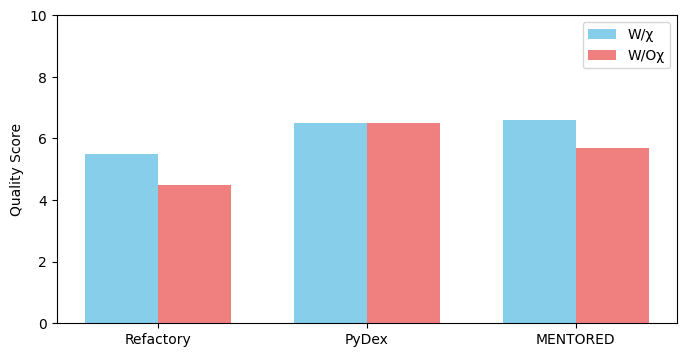
\includegraphics[width=1.0\linewidth]{quality.png}
            \caption{Comparison of Feedback Quality}
            \label{fig:quality}
        \end{figure}

        % 피드백(패치)의 품질을 측정하기 위해 Pylint 라이브러리를 사용하였습니다. Pylint\footnote{\url{https://www.pylint.org}}는 Python 정적 분석 도구로서, 다섯가지 카테고리(fatal, error, warning, convention, refactor)를 종합적으로 평가하여 코드의 품질을 정량적으로 측정하며 많은 연구에서 사용되고 있습니다 \cite{siddiq2024quality, horschig2018java, apostolidis2023evaluation, agarwal2020quality}. Fig \ref{fig:quality} shows a comparison of feedback  quality. The quality score is out of 10. correct program이 제공되는 $W/\;\chi$ 조건에서 \textsc{Mentored}는 6.6점으로 가장 높은 품질을 기록하였으며, \textsc{PyDex}는 6.5점, \textsc{Refactory}는 5.5점을 기록했습니다. 반면, correct program이 제공되지 않는 $W/O\;\chi$ 조건에서는 \textsc{PyDex}가 6.5점으로 가장 높은 점수를 받았지만, \textsc{Mentored}는 5.7점으로 두 번째로 높은 점수를 기록하였고, \textsc{Refactory}는 4.5점에 그쳤습니다. 이러한 결과는 \textsc{Mentored}가 correct program이 있는 상황에서 가장 우수한 품질을 제공하며, \textsc{PyDex}보다도 뛰어난 성능을 보인다는 것을 나타냅니다. 비록 $W/O;\chi$ 조건에서 \textsc{PyDex}가 약간 더 높은 점수를 얻었지만, \textsc{Mentored}는 여전히 안정적인 품질을 유지하였습니다. \textsc{Mentored}의 주요 강점은 피드백 생성 과정에서 대형 언어 모델(LLM)에 의존하지 않는다는 것입니다. \textsc{PyDex}는 LLM를 기반으로 코드를 생성하기 때문에 높은 성능을 보일 수 있지만, LLM의 불안정성과 데이터 편향 문제로 인해 생성된 피드백의 정확성과 일관성이 저하될 수 있습니다 \cite{zhang2024pydex}. 또한, LLM은 블랙박스 방식으로 동작하여 \textsc{PyDex}가 생성하는 수정 사항의 논리적 근거를 설명하거나 과정을 투명하게 제시하기 어렵습니다. 이에 반해, \textsc{Mentored}는 피드백 생성 과정이 투명하며, 학생들이 자신의 오류를 이해하는 데 도움이 되는 해석 가능한 피드백을 제공합니다. 추가로, \textsc{PyDex}는 데이터 누출의 위험이 있어 평가 결과의 신뢰성을 저하시킬 수 있습니다. 반면, \textsc{Mentored}는 자체 알고리즘을 통해 이러한 문제를 방지하고, 데이터 의존성을 감소시켜 더 안정적이고 신뢰할 수 있는 피드백을 제공합니다.
        To measure the quality of feedback, we used the Pylint library. Pylint\footnote{\url{https://www.pylint.org}} is a static analysis tool for Python that comprehensively evaluates code across five categories (fatal, error, warning, convention, refactor) to quantitatively assess quality. It has been widely employed in numerous studies \cite{siddiq2024quality, horschig2018java, apostolidis2023evaluation, agarwal2020quality}. Fig \ref{fig:quality} presents a comparison of feedback quality. The quality score is out of 10. In the $W/\;\chi$ condition where correct programs are provided, \textsc{Mentored} performed the highest quality score of 6.6, followed by \textsc{PyDex} with 6.5 and \textsc{Refactory} with 5.5. On the other hand, in $W/O\;\chi$, \textsc{PyDex} performed the highest score of 6.5, while \textsc{Mentored} attained a second highest score of 5.7, and \textsc{Refactory} scored 4.5. These results indicate that \textsc{Mentored} delivers superior quality in $W/\;\chi$, outperforming \textsc{PyDex}. Although \textsc{PyDex} obtained a slightly higher score in $W/O\;\chi$, \textsc{Mentored} still maintained consistently high quality. A key strength of \textsc{Mentored} is that it does not rely on LLM. While \textsc{PyDex} can exhibit high performance by generating code based on LLM, the instability of LLM and issues of data bias can compromise the accuracy and consistency of the generated feedback \cite{zhang2024pydex}. Additionally, since LLM operate as black boxes, it is challenging to explain the logical basis for the modifications generated by \textsc{PyDex} or to present the process transparently. In contrast, \textsc{Mentored} ensures transparency in the feedback generation process and provides interpretable feedback that aids students in understanding their mistakes. Furthermore, \textsc{PyDex} carries the risk of data leakage, which can undermine the reliability of the evaluation results. Conversely, \textsc{Mentored} mitigates such issues through its proprietary algorithms, reduces data dependency, and provides more stable and reliable feedback.

        \begin{tcolorbox}
            \textbf{Answer to RQ3.}
            % \textsc{Mentored}는 correct programs가 제공되는 조건에서 최고 수준의 피드백 품질을 달성했으며, correct programs가 없는 상황에서도 안정적으로 높은 품질의 피드백을 제공합니다. 비록 \textsc{PyDex}가 correct programs가 없는 상황에서 더 높은 성능을 보이지만, \textsc{Mentored}는 블랙박스 방식의 LLM 기반 \textsc{PyDex}와 달리 투명하고 해석 가능한 피드백을 제공합니다. 이러한 피드백은 특히 교육 환경에서 학생들의 학습을 더욱 효과적으로 지원합니다.
            \textsc{Mentored} achieved top feedback quality with correct programs and maintained high quality even without. While \textsc{PyDex} performs better without correct programs, \textsc{Mentored} offers more transparent and interpretable feedback than the black-box LLM-based \textsc{PyDex}. This feedback is especially useful in educational environments, effectively supporting student learning.
        \end{tcolorbox}

        

\section{Threats to Validity}
    To support a more reasonable comparison, we reimplemented \textsc{PyDex} which is the most recent and competitive approach to the best of our knowledge. However, \textsc{PyDex} are not publicly available, so we tried to follow the original paper as much as possible, but there may be some differences in the implementation. For instance, the original LLM engine of \textsc{PyDex} is no longer supported, so we used the closest later supported engine \textit{gpt-3.5-turbo}. This change may introduce a threat to internal validity, potentially affecting the performance of \textsc{PyDex}. To mitigate this threat, we have made the source code of the reimplemented \textsc{PyDex} publicly available on Github for peer-review to reproduce our results and verify the correctness of the implementation. Additionally, our proposed method, \textsc{Mentored}, is also publicly available on Github at \ref{tool}.

    There may be threats to external validity due to the datasets and evaluation metrics chosen for the experiments. To minimize this threat, we selected various datasets from real university programming assignments and online judges, as used in existing approaches. Additionally, we chose evaluation metrics that are commonly used in AFG approaches.

    Finally, we acknowledge potential threats to conclusion validity, as statistical variations could influence the outcomes of our comparisons. To ensure that our results are robust and reliable, we performed multiple runs of 100 trials, accounting for possible variations due to the inherent randomness of GP.



\section{Conclusion}
    % Correct programs에 의존하는 기존 AFG 기술들은 correct programs가 없는 상황에서 효과적으로 작동하지 못하는 한계가 있습니다. 본 논문에서는 이러한 한계를 극복하기 위해 correct programs 없이도 다양한 피드백을 생성할 수 있는 새로운 approach인 \textsc{Mentored}를 제안했습니다. \textsc{Mentored}의 핵심은 유전 프로그래밍을 활용하여 다양한 패치를 생성하고, 반복적인 탐색 과정을 통해 최적의 수정안을 찾는 것입니다. 실제 학생들의 프로그래밍 과제를 통해 평가한 결과, \textsc{Mentored}는 기존 기술들과 비교해 더 다양하고 고품질의 피드백을 생성할 수 있음을 확인했습니다. 특히, \textsc{Mentored}는 유전 프로그래밍의 수정 과정을 투명하게 제공하여 학생들이 자신의 오류를 단계별로 이해하고 수정할 수 있도록 돕는 해석 가능한 피드백을 제공합니다. 또한, 프로그램의 구조를 유지하면서도 다양한 수정안을 제시함으로써 학생들이 여러 해결책을 경험하고 학습할 수 있게 합니다. 이러한 강점은 프로그래밍 교육을 효과적으로 개선하고, 강사의 수고를 줄이며, 학생들의 프로그래밍 역량을 향상시키는 데 기여할 것입니다.
    Existing AFG techniques that rely on correct programs face limitations in generating feedback when correct programs are unavailable. In this paper, we propose a new approach, \textsc{Mentored}, that can generate diverse feedback without rely on correct programs. The key idea of \textsc{Mentored} is to utilize genetic programming to generate diverse patches and find the optimal solution through iterative repair processes. Through evaluations on real student programming assignments, we demonstrated that \textsc{Mentored} can produce more diverse and higher-quality feedback compared to existing techniques. Notably, \textsc{Mentored} provides interpretable feedback by transparently providing the iterative repair process, allowing students to understand and repair their faults step by step. Moreover, while maintaining the structure of the original(wrong) program, it sometimes suggests solutions with different structures, helping students learn from and experience various solutions. These strengths contribute to improving programming education, reducing the instructors' workload, and enhancing students' programming skills.



\section{Data Availability} \label{tool}
    Our \textsc{Mentored} tool implementation of the approach is available at \url{https://github.com/dwchoi95/MENTORED}



\section*{Acknowledgment}
    This work was supported by the Institute of Information \& Communications Technology Planning \& Evaluation(IITP) grant funded by the Korea government(MSIT) (No.RS-2024-00438686, Development of software reliability improvement technology through identification of abnormal open sources and automatic application of DevSecOps)


\bibliographystyle{IEEEtran}
\bibliography{references}



\end{document}
